\documentclass[12pt,a4paper]{report}

% ============================================================
% PACKAGES (100% STANDAR OVERLEAF / PDFLATEX)
% ============================================================
\usepackage[utf8]{inputenc}
\usepackage[T1]{fontenc}
\usepackage[indonesian]{babel}
\usepackage{mathptmx} % Times New Roman untuk teks & matematika
\usepackage[scaled=0.85]{couriers} % Courier ringkas agar teks kode di tabel & paragraf tidak meluber
\usepackage[top=3cm,bottom=3cm,left=4cm,right=3cm]{geometry}
\usepackage{setspace}
\usepackage{amsmath,amssymb}
\usepackage{graphicx}
\usepackage{float}
\usepackage{booktabs}
\usepackage{tabularx}
\usepackage{array}
\usepackage[table]{xcolor}
\usepackage{caption}
\usepackage{titlesec}
\usepackage{fancyhdr}
\usepackage{enumitem}
\usepackage{tcolorbox}
\usepackage{microtype}
\usepackage{xurl}
\usepackage[hidelinks]{hyperref}

% ============================================================
% KONFIGURASI WARNA, TIPOGRAFI, DAN TATA LETAK
% ============================================================
\graphicspath{{images/}}
\onehalfspacing
\setlength{\parindent}{1cm}
\setlength{\parskip}{4pt}
\emergencystretch=2em

\definecolor{HeaderBlue}{HTML}{4F81BD}
\definecolor{LightRow}{HTML}{F2F5F9}
\definecolor{HighlightRow}{HTML}{E8EEF7}
\definecolor{CodeColor}{HTML}{1E3A5F}
\definecolor{MutedGray}{HTML}{555555}

% Helper penulisan kode inline yang rapi (mewarisi ukuran font sekitar secara aman)
\DeclareRobustCommand{\code}[1]{\texttt{\textcolor{CodeColor}{#1}}}

% Kolom tabel terstruktur tanpa rata kiri-kanan berlebihan
\newcolumntype{P}[1]{>{\raggedright\arraybackslash}p{#1}}
\newcolumntype{M}[1]{>{\centering\arraybackslash}p{#1}}
\newcolumntype{L}{>{\raggedright\arraybackslash}X}
\newcolumntype{C}{>{\centering\arraybackslash}X}
\newcommand{\thdr}[1]{\textcolor{white}{\textbf{#1}}}

% Format judul BAB (Terpusat, 14pt, Bold, Hitam)
\titleformat{\chapter}[display]
  {\normalfont\fontsize{14}{17}\selectfont\bfseries\centering}
  {BAB \thechapter}
  {2pt}
  {\MakeUppercase}
\titlespacing*{\chapter}{0pt}{-12pt}{14pt}

% Format Subbab & Sub-subbab (Rata Kiri, 12pt, Bold, Hitam)
\titleformat{\section}
  {\normalfont\fontsize{12}{15}\selectfont\bfseries}
  {\thesection}
  {0.7em}
  {}
\titlespacing*{\section}{0pt}{12pt}{4pt}

\titleformat{\subsection}
  {\normalfont\fontsize{12}{15}\selectfont\bfseries}
  {\thesubsection}
  {0.7em}
  {}
\titlespacing*{\subsection}{0pt}{8pt}{3pt}

% Format Caption Tabel & Gambar
\captionsetup{
  font=small,
  labelfont=bf,
  labelsep=space,
  skip=6pt
}
\captionsetup[table]{position=top, justification=raggedright, singlelinecheck=false}
\captionsetup[figure]{position=bottom, justification=centering}

% Header & Footer
\pagestyle{fancy}
\fancyhf{}
\fancyhead[R]{\fontsize{9}{11}\selectfont\itshape\textcolor{MutedGray}{Laporan Team-Based Project (TBP) Data Mining --- E-Commerce Customer Churn (SHAP)}}
\fancyfoot[C]{\fontsize{10}{12}\selectfont\textcolor{MutedGray}{\thepage}}
\renewcommand{\headrulewidth}{0pt}
\renewcommand{\footrulewidth}{0pt}

\fancypagestyle{plain}{
  \fancyhf{}
  \fancyfoot[C]{\fontsize{10}{12}\selectfont\textcolor{MutedGray}{\thepage}}
  \renewcommand{\headrulewidth}{0pt}
}

% Kotak placeholder screenshot Streamlit
\tcbset{
  screenshotbox/.style={
    colback=LightRow,
    colframe=HeaderBlue,
    boxrule=0.8pt,
    arc=3pt,
    top=14pt,
    bottom=14pt,
    left=12pt,
    right=12pt,
    halign=center
  }
}

% Label Bahasa Indonesia untuk TOC/LOT/LOF
\addto\captionsindonesian{
  \renewcommand{\contentsname}{DAFTAR ISI}
  \renewcommand{\listtablename}{DAFTAR TABEL}
  \renewcommand{\listfigurename}{DAFTAR GAMBAR}
  \renewcommand{\tablename}{Tabel}
  \renewcommand{\figurename}{Gambar}
}

% ============================================================
% MULAI DOKUMEN
% ============================================================
\begin{document}

% ------------------------------------------------------------
% HALAMAN SAMPUL
% ------------------------------------------------------------
\begin{titlepage}
  \singlespacing
  \centering
  \vspace*{0.1cm}
  {\fontsize{14}{18}\selectfont\bfseries
    LAPORAN TEAM-BASED PROJECT (TBP)\\
    MATA KULIAH DATA MINING\par}

  \vspace{0.6cm}
  {\fontsize{14}{19}\selectfont\bfseries
    SISTEM PREDIKSI \textit{E-COMMERCE CUSTOMER CHURN}\\
    MENGGUNAKAN KOMPARASI ALGORITMA KLASIFIKASI\\
    BERBASIS \textit{EXPLAINABLE AI} (SHAP)\par}

  \vspace{0.8cm}
  
\includegraphics[width=3.6cm]{logo_uns.png}

  \vspace{0.8cm}
  {\fontsize{12}{16}\selectfont
    \textbf{Dosen Pengampu:}\\
    DR. Wiranto M.KOM., M.CS.\par}

  \vspace{0.6cm}
  {\fontsize{12}{16}\selectfont\textbf{Disusun Oleh --- Kelompok 6:}\par}
  \vspace{0.2cm}

  {\renewcommand{\arraystretch}{1.15}
  \begin{tabular}{@{}p{7.2cm}l@{}}
    1. Adrian Alviano Susatyo & L0124001 \\
    2. Daniel Ferdian Napitupulu & L0124008 \\
    3. Radit Alfa Anugerah Bombing & L0124116 \\
    4. Valentino Joan Caesar & L0124121 \\
    5. Aerio Ade Putra & L0124128 \\
  \end{tabular}}

  \vspace{0.5cm}
  {\fontsize{10}{14}\selectfont
    \textbf{Repositori GitHub:}\\
    \url{https://github.com/aerioade/ecommerce-customer-churn-prediction}\par}

  \vfill
  {\fontsize{12}{16}\selectfont\bfseries
    PROGRAM STUDI INFORMATIKA\\
    FAKULTAS TEKNOLOGI DAN SAINS DATA\\
    UNIVERSITAS SEBELAS MARET\\
    2026\par}
\end{titlepage}

% ------------------------------------------------------------
% HALAMAN DEPAN (ROMAN PAGE NUMBERING)
% ------------------------------------------------------------
\pagenumbering{roman}
\tableofcontents
\clearpage
\listoftables
\clearpage
\listoffigures
\clearpage

% ------------------------------------------------------------
% ISI LAPORAN (ARABIC PAGE NUMBERING)
% ------------------------------------------------------------
\pagenumbering{arabic}

% ============================================================
% BAB 1: PENDAHULUAN
% ============================================================
\chapter{Pendahuluan}

\section{Latar Belakang}

Pertumbuhan pesat industri perdagangan elektronik (\textit{e-commerce}) telah mengubah pola transaksi konsumen secara fundamental sekaligus meningkatkan intensitas persaingan antarplatform digital. Dengan rendahnya biaya perpindahan (\textit{switching cost}) di pasar digital, pelanggan dapat dengan mudah berpindah ke platform kompetitor apabila mengalami ketidakpuasan layanan, keterlambatan pengiriman, atau penurunan relevansi penawaran (Hantash et al., 2026). Fenomena berhentinya pelanggan dari suatu platform transaksi---yang dikenal sebagai \textit{customer churn}---merupakan ancaman langsung terhadap stabilitas pendapatan dan keberlanjutan bisnis jangka panjang. Secara ekonomis, biaya untuk mengakuisisi pelanggan baru di industri digital diperkirakan mencapai \textbf{5 hingga 25 kali lebih mahal} dibandingkan biaya mempertahankan pelanggan yang sudah ada (\textit{existing customers}). Oleh karena itu, kemampuan mendeteksi risiko \textit{churn} secara dini sebelum pelanggan benar-benar meninggalkan platform menjadi kebutuhan strategis yang krusial bagi tim \textit{Customer Relationship Management} (CRM).

Meskipun penerapan \textit{machine learning} untuk prediksi \textit{customer churn} telah banyak dikaji, terdapat tiga permasalahan utama yang membatasi pemanfaatannya secara praktis di sektor \textit{e-commerce}. \textbf{Pertama}, dominasi penelitian prediksi \textit{churn} masih berpusat pada sektor telekomunikasi dan perbankan ritel, sehingga validasi langsung pada karakteristik perilaku transaksi \textit{e-commerce}---seperti jarak gudang ke rumah, riwayat komplain, jumlah perangkat terdaftar, dan respons terhadap \textit{cashback}---masih relatif terbatas (Hantash et al., 2026; Khan et al., 2026). \textbf{Kedua}, dalam praktik pemodelan data riil, masih sering ditemukan kelemahan metodologis berupa kebocoran data (\textit{data leakage}) akibat tidak dihapuskannya rekaman duplikat sebelum pemisahan data maupun proses imputasi dan normalisasi yang dilakukan pada keseluruhan dataset sebelum \textit{train-test split}. Selain itu, data \textit{churn} umumnya bersifat tidak seimbang (\textit{imbalanced}), sehingga penggunaan teknik \textit{oversampling} sintetis secara kurang tepat berisiko mengubah distribusi alami perilaku pelanggan. \textbf{Ketiga}, model \textit{ensemble} modern berperforma tinggi seperti \textit{Random Forest} dan \textit{XGBoost} cenderung bersifat kotak hitam (\textit{black-box}). Tanpa mekanisme penjelasan yang transparan, tim bisnis dan pemasaran tidak dapat memahami \textit{mengapa} seorang pelanggan diprediksi akan \textit{churn}, sehingga skor prediksi sulit diterjemahkan menjadi tindakan retensi yang tepat sasaran (Inkesar, 2026; Lundberg \& Lee, 2017).

Berdasarkan uraian permasalahan tersebut, proyek ini mengadopsi pendekatan integratif yang menggabungkan analisis kasus mendalam (\textit{Case Method}) dengan pembangunan solusi produk nyata (\textit{Team-Based Project}). Melalui analisis kasus perilaku pelanggan \textit{e-commerce}, tim merancang alur \textit{Data Mining} yang ketat terhadap \textit{data leakage}, membandingkan tiga algoritma klasifikasi dari paradigma berbeda (\textbf{Logistic Regression}, \textbf{Random Forest}, dan \textbf{XGBoost}), serta mengintegrasikan kerangka kerja \textbf{\textit{Explainable AI}} (\textbf{SHAP --- SHapley Additive exPlanations}) untuk membedah faktor pendorong \textit{churn} secara global maupun individual. Selanjutnya, hasil analitik tersebut dioperasionalisasikan menjadi sebuah \textbf{produk aplikasi web dashboard interaktif berbasis Streamlit} yang dilengkapi sistem \textbf{\textit{3-Tier Risk Stratification}} (\textit{High}, \textit{Medium}, dan \textit{Low Risk}) serta rekomendasi aksi retensi otomatis bagi tim manajemen dan CRM.

\section{Rumusan Masalah}

Berdasarkan latar belakang di atas, rumusan masalah dalam \textit{Team-Based Project} ini adalah sebagai berikut:
\begin{enumerate}[leftmargin=0.8cm, itemsep=2pt]
  \item Bagaimana merancang alur \textit{preprocessing} dan pemodelan klasifikasi \textit{e-commerce customer churn} yang bebas dari kebocoran data (\textit{data leakage}) serta mampu menangani ketidakseimbangan kelas (\textit{class imbalance}) secara alami tanpa \textit{oversampling} sintetis?
  \item Bagaimana perbandingan performa tiga algoritma klasifikasi dari paradigma berbeda---yaitu \textbf{Logistic Regression} (\textit{linear baseline}), \textbf{Random Forest} (\textit{ensemble bagging}), dan \textbf{XGBoost} (\textit{ensemble boosting})---ditinjau dari metrik \textit{Accuracy, Precision, Recall, Specificity, F1-Score, False Positive Rate} (FPR), dan \textit{ROC-AUC}?
  \item Faktor perilaku pelanggan apa saja yang paling dominan memengaruhi keputusan \textit{churn} pada platform \textit{e-commerce} berdasarkan analisis global dan lokal \textbf{SHAP}, serta bagaimana konsistensinya terhadap \textit{feature importance} bawaan model berbasis pohon (\textit{dual validation})?
  \item Bagaimana mengoperasionalisasikan model prediksi terbaik dan penjelasan SHAP ke dalam \textit{prototype web dashboard} interaktif dengan mekanisme \textbf{\textit{3-Tier Risk Stratification}} agar dapat menghasilkan rekomendasi retensi yang aplikatif bagi tim CRM?
\end{enumerate}

\section{Tujuan Proyek}

Tujuan dari pelaksanaan proyek ini adalah:
\begin{enumerate}[leftmargin=0.8cm, itemsep=2pt]
  \item Membangun \textit{pipeline Data Mining end-to-end} yang reproduksibel dan menerapkan protokol anti-\textit{data leakage} secara ketat mulai dari standarisasi kategori, deduplikasi data, \textit{stratified train-test split}, hingga transformasi fitur dalam \code{ColumnTransformer} dan \code{Pipeline}.
  \item Melatih, mengoptimasi (\textit{hyperparameter tuning} berbasis \textit{5-Fold Stratified Cross-Validation}), dan membandingkan secara objektif kinerja algoritma Logistic Regression, Random Forest, dan XGBoost untuk memperoleh model klasifikasi \textit{churn} terbaik.
  \item Memberikan transparansi keputusan model (\textit{model interpretability}) baik pada tingkat global maupun individual pelanggan menggunakan \textbf{SHAP}, disertai validasi ganda (\textit{dual validation}) terhadap \textit{Tree Gain/Gini Importance}.
  \item Mengembangkan \textit{prototype} aplikasi web interaktif berbasis \textbf{Streamlit} yang mendukung simulasi prediksi individual (dengan \textit{SHAP Waterfall Plot}), prediksi massal (\textit{batch prediction} via unggah CSV/Excel), analitik komparasi 3 model, eksplorasi data (EDA), dan rekomendasi aksi retensi otomatis berbasis \textit{3-Tier Risk Stratification}.
\end{enumerate}

\section{Ruang Lingkup dan Batasan Proyek}

Agar pelaksanaan proyek tetap terfokus, terukur, dan konsisten dengan kondisi data aktual, ditetapkan batasan-batasan sebagai berikut:
\begin{enumerate}[leftmargin=0.8cm, itemsep=2pt]
  \item \textbf{Skema Dataset Aktual:} Penelitian menggunakan dataset sekunder \code{data\_\allowbreak ecommerce\_\allowbreak customer\_\allowbreak churn.csv} yang terdiri atas \textbf{3.941 baris mentah} dan \textbf{11 kolom} (10 fitur prediktor perilaku/demografi dan 1 variabel target biner \code{Churn}), tanpa melibatkan atribut eksternal yang tidak tersedia dalam dataset (seperti \code{CustomerID}, \code{Gender}, atau log klik \textit{real-time}).
  \item \textbf{Algoritma Pembanding:} Pemodelan difokuskan pada komparasi tiga paradigma klasifikasi yang saling melengkapi, yaitu Logistic Regression, Random Forest, dan XGBoost, dengan nilai benih acak tetap (\code{RANDOM\_STATE = 42}) untuk menjamin reproduksibilitas penuh.
  \item \textbf{Penanganan Imbalance, Outlier, dan Dimensi Fitur:} Ketidakseimbangan kelas ditangani menggunakan pembobotan kelas internal (\textit{cost-sensitive learning}: \code{class\_weight='balanced'} dan \code{scale\_pos\_weight}) \textbf{tanpa} SMOTE/resampling sintetis. Reduksi dimensi seperti PCA \textbf{tidak digunakan} demi menjaga keterbacaan nama fitur asli pada grafik SHAP. \textit{Outlier} yang terdeteksi dengan metode IQR didokumentasikan pada tahap EDA dan tidak dihapus agar variasi perilaku pelanggan nyata tetap terjaga.
  \item \textbf{Lingkup Deployment:} Implementasi produk akhir berupa \textit{prototype web dashboard} lokal berbasis Streamlit yang menggunakan artefak model terlatih (\code{.joblib}) dan ringkasan evaluasi terstruktur (\code{.json}), tanpa integrasi ke basis data produksi (\textit{live production database}) perusahaan tertentu.
\end{enumerate}

\section{Manfaat dan Target Luaran Proyek (\textit{Deliverables})}

Proyek ini memberikan manfaat baik secara akademis (penerapan metodologi \textit{Data Mining} anti-\textit{data leakage} dan \textit{Explainable AI}) maupun secara praktis bagi pengambil keputusan bisnis \textit{e-commerce} dalam memprioritaskan anggaran retensi pelanggan secara terukur. Selaras dengan ketentuan \textit{Team-Based Project} (TBP) mata kuliah Data Mining yang berorientasi produk (\textit{project/product-centered learning}), proyek ini menargetkan enam luaran (\textit{deliverables}) wajib sebagaimana dirangkum pada Tabel~\ref{tab:deliverables}.

\begin{table}[H]
  \centering
  \caption{Target Luaran (\textit{Deliverables}) Wajib \textit{Team-Based Project}}
  \label{tab:deliverables}
  \renewcommand{\arraystretch}{1.28}
  \setlength{\tabcolsep}{4pt}
  \footnotesize
  \begin{tabularx}{\textwidth}{@{}M{0.6cm} P{2.9cm} L P{3.5cm}@{}}
    \toprule
    \rowcolor{HeaderBlue}
    \thdr{No} & \thdr{Luaran (\textit{Deliverable})} & \thdr{Spesifikasi Teknis \& Isi} & \thdr{Format / Lokasi} \\
    \midrule
    1 & \textbf{Dataset Bersih \& Terdokumentasi} & Dataset mentah (3.941 baris) serta partisi bersih hasil standarisasi kategori, deduplikasi, dan \textit{stratified split} 80:20 (\code{train\_data.csv} \& \code{test\_data.csv}), lengkap dengan kamus 11 atribut. & \code{.csv}\newline(\code{data/raw/},\newline\code{data/processed/}) \\
    \rowcolor{LightRow}
    2 & \textbf{Kode Program Modular \& Notebook} & \textit{Codebase} Python modular (\code{config.py}, \code{data\_loader.py}, \code{eda.py}, \code{preprocessing.py}, \code{train.py}, \code{explainability.py}, \code{risk\_engine.py}) serta notebook eksperimen \textit{end-to-end}. & \code{.py}, \code{.ipynb}\newline(\code{src/}, \code{notebooks/}) \\
    3 & \textbf{Artefak Model Terlatih \& Evaluasi} & File serialisasi \textit{pipeline} lengkap (\code{Preprocessor + Classifier}) untuk 3 algoritma, model terbaik, latar belakang SHAP, serta laporan metrik/EDA/SHAP terstruktur. & \code{.joblib}, \code{.json}\newline(\code{models/}, \code{artifacts/}) \\
    \rowcolor{LightRow}
    4 & \textbf{\textit{Prototype / Web Dashboard} Interaktif} & Aplikasi web berbasis Streamlit dengan 4 modul utama: Prediksi Individual + SHAP Lokal, \textit{Batch Prediction} CSV/Excel, Analitik Komparasi 3 Model, dan Ringkasan EDA. & \textbf{Web App}\newline(\code{app/\allowbreak streamlit\_app.py}) \\
    5 & \textbf{Laporan Proyek Akademis} & Laporan tertulis sistematis Bab 1 s.d. Bab 5 yang memuat manajemen proses tim, landasan matematis, analisis hasil eksperimen, interpretasi SHAP, dan referensi ilmiah. & \code{.tex} / \code{.docx} / \code{.pdf} \\
    \rowcolor{LightRow}
    6 & \textbf{Slide Presentasi \& Skenario \textit{Live Demo}} & Materi presentasi tim yang ringkas disertai skenario demonstrasi langsung penggunaan \textit{web dashboard} (simulasi pelanggan High/Low Risk dan unggah \textit{batch} CSV). & \code{.pptx} / \code{.pdf} \\
    \bottomrule
  \end{tabularx}
\end{table}

% ============================================================
% BAB 2: TINJAUAN PUSTAKA DAN LANDASAN TEORI
% ============================================================
\chapter{Tinjauan Pustaka dan Landasan Teori}

\section{Tinjauan Penelitian Terdahulu (\textit{State of the Art})}

Kajian terhadap literatur ilmiah terkini pada periode 2024--2026 menunjukkan tren kuat dalam pergeseran pendekatan prediksi \textit{customer churn} dari sekadar pemodelan klasifikasi konvensional menuju sistem pendukung keputusan berbasis \textit{ensemble machine learning} dan \textit{Explainable AI} (SHAP). Ringkasan komparasi empat studi acuan utama disajikan pada Tabel~\ref{tab:sota}.

\begin{table}[H]
  \centering
  \caption{Matriks Perbandingan Penelitian Terdahulu (\textit{State of the Art})}
  \label{tab:sota}
  \renewcommand{\arraystretch}{1.28}
  \setlength{\tabcolsep}{3.5pt}
  \scriptsize
  \begin{tabularx}{\textwidth}{@{}M{0.5cm} P{2.2cm} P{1.9cm} L L L@{}}
    \toprule
    \rowcolor{HeaderBlue}
    \thdr{No} & \thdr{Peneliti \& Publikasi} & \thdr{Domain \& Dataset} & \thdr{Metode \& Penanganan Imbalance} & \thdr{Hasil Utama \& Peran XAI} & \thdr{Keterbatasan / Celah (\textit{Gap})} \\
    \midrule
    1 & \textbf{Khan et al. (2026)} \textit{MDPI Information, 17(9), 886 (Scopus)} & \textit{E-Commerce} (50.000 rekaman transaksi \& performa web) & XGBoost dengan \textit{stratified split}, rekayasa skor kualitas teknis \& informasi (WPIS), validasi fitur ganda. & Akurasi $\approx$92,1\%, AUC-ROC 0,93 (churn), F1 0,86 (\textit{high-risk}); SHAP memvalidasi \textit{gain importance} \& mendukung stratifikasi risiko MIS. & Memerlukan metrik telemetri web khusus (\textit{session friction}, IQDi) yang tidak selalu tersedia pada dataset transaksi standar. \\
    \rowcolor{LightRow}
    2 & \textbf{Inkesar (2026)} \textit{IEEE Access, Vol. 14, pp. 119355--119383 (Scopus)} & \textit{Customer Churn} Industri (data campuran numerik \& kategorikal) & \textit{Density-Regularized Oversampling} (SMOTE-ENC) + model klasifikasi \& kerangka SHAP. & Mengurangi tumpang tindih \textit{noise} sampel minoritas \& meningkatkan transparansi faktor pendorong \textit{churn} bagi tim CRM. & Berfokus pada \textit{oversampling} sintetis; belum mengevaluasi strategi bobot kelas alami yang terintegrasi ke \textit{dashboard} interaktif. \\
    3 & \textbf{Ahmad et al. (2024)} \textit{IEEE Access, Vol. 12, pp. 1865--1879 (Scopus)} & Analisis Kepribadian \& \textit{Churn} Pelanggan (tidak seimbang) & \textit{Bagging} (RF), \textit{Boosting} (XGBoost, LightGBM, AdaBoost), \& \textit{Stacking} (HSLR) dengan SMOTE \& CTGAN. & Model hibrida \textit{ensemble} + SMOTE mencapai Akurasi 94,06\%, F1 94,05\%, dan ROC 0,984; membuktikan keunggulan \textit{ensemble} atas model tunggal. & Tidak menyertakan modul \textit{Explainable AI} (SHAP) lokal per individu maupun antarmuka operasional \textit{web dashboard} untuk pengguna bisnis. \\
    \rowcolor{LightRow}
    4 & \textbf{Hantash et al. (2026)} \textit{JIDMIS, Vol. 3(7s), pp. 1023--1041 (Pendukung)} & Telekomunikasi \& Perbankan Ritel (17.032 rekaman gabungan) & Komparasi 5 model (LR, RF, GB, XGBoost, LightGBM), SMOTE pada data latih, SHAP, \& \textit{K-Means}. & \textit{Gradient Boosting} meraih F1 0,55 \& AUC 0,80; XGBoost akurasi tertinggi 74,2\%, LR terendah (66,2\%). SHAP mengonfirmasi sinyal perilaku. & Peneliti secara eksplisit mencatat hasil telko/perbankan belum dapat digeneralisasi ke sektor \textit{e-commerce} tanpa validasi data \textit{e-commerce} aktual. \\
    \bottomrule
  \end{tabularx}
\end{table}

\subsection*{Sintesis Celah Penelitian (\textit{Research Gap}) dan Posisi Proyek}
\noindent Berdasarkan sintesis literatur pada Tabel~\ref{tab:sota}, dapat diidentifikasi tiga celah utama yang menjadi pijakan proyek ini:
\begin{enumerate}[leftmargin=0.8cm, itemsep=2pt]
  \item \textbf{Keterbatasan Validasi Lintas Sektor pada \textit{E-Commerce}:} Sebagaimana ditegaskan oleh Hantash et al. (2026), penelitian \textit{churn} masih didominasi data telekomunikasi dan perbankan, sehingga diperlukan pemodelan langsung pada atribut perilaku \textit{e-commerce} aktual (seperti jarak pengiriman \code{WarehouseToHome}, kategori pesanan favorit \code{PreferedOrderCat}, skor kepuasan \code{SatisfactionScore}, dan riwayat komplain langsung \code{Complain}).
  \item \textbf{Kebutuhan Evaluasi Anti-\textit{Data Leakage} Tanpa Distorsi Data Sintetis:} Mayoritas penelitian terdahulu (Ahmad et al., 2024; Inkesar, 2026; Hantash et al., 2026) bergantung pada \textit{oversampling} sintetis seperti SMOTE. Proyek ini menguji pendekatan \textit{cost-sensitive learning} (\code{class\_weight='balanced'} dan \code{scale\_pos\_weight}) yang menjaga keaslian distribusi data dalam \textit{pipeline} anti-\textit{data leakage} yang ketat.
  \item \textbf{Kebaruan Terapan (\textit{Applied Novelty}):} Menggabungkan validasi ganda SHAP vs \textit{Tree Feature Importance} dan konsep stratifikasi risiko dari Khan et al. (2026) langsung ke dalam sebuah \textbf{produk \textit{web dashboard} Streamlit siap pakai} yang menyediakan simulasi individu, \textit{SHAP Waterfall Plot}, prediksi massal (\textit{batch}), dan rekomendasi aksi retensi otomatis dalam satu antarmuka terpadu.
\end{enumerate}

\section{Landasan Teori dan Formulasi Matematis}

\subsection{\textit{E-Commerce Customer Churn} dan Klasifikasi Biner}

\textit{Customer churn} pada \textit{e-commerce} didefinisikan sebagai kondisi ketika pelanggan menghentikan aktivitas pembelian atau meninggalkan platform dalam suatu periode observasi. Dalam kerangka \textit{Data Mining}, permasalahan prediksi \textit{churn} dirumuskan sebagai tugas \textbf{klasifikasi biner (\textit{binary classification})}, di mana setiap observasi pelanggan direpresentasikan oleh vektor fitur $\mathbf{x}_i \in \mathbb{R}^d$ dan dipetakan menuju label target diskrit $y_i \in \{0, 1\}$, dengan $y_i = 0$ menyatakan pelanggan bertahan (\textit{Non-Churn}) dan $y_i = 1$ menyatakan pelanggan berhenti (\textit{Churn}). Model klasifikasi bertujuan mempelajari fungsi probabilitas bersyarat $p_i = P(y_i = 1 \mid \mathbf{x}_i) \in [0, 1]$.

\subsection{Deteksi \textit{Outlier} (\textit{Interquartile Range}) dan Standarisasi \textit{Z-Score}}

Metode \textit{Interquartile Range} (IQR) digunakan pada tahap \textit{Exploratory Data Analysis} (EDA) untuk mengidentifikasi nilai ekstrem pada fitur numerik kontinu tanpa mengasumsikan distribusi normal. Jika $Q_1$ adalah kuartil pertama (persentil ke-25) dan $Q_3$ adalah kuartil ketiga (persentil ke-75), maka rentang antarkuartil dan batas deteksi \textit{outlier} dirumuskan pada Persamaan~\eqref{eq:iqr}--\eqref{eq:ub}:
\begin{equation}
  \mathrm{IQR} = Q_3 - Q_1
  \label{eq:iqr}
\end{equation}
\begin{equation}
  \mathrm{Lower\ Bound} = Q_1 - 1{,}5 \times \mathrm{IQR}
  \label{eq:lb}
\end{equation}
\begin{equation}
  \mathrm{Upper\ Bound} = Q_3 + 1{,}5 \times \mathrm{IQR}
  \label{eq:ub}
\end{equation}

Suatu pengamatan $x$ diklasifikasikan sebagai \textit{outlier} apabila $x < \mathrm{Lower\ Bound}$ atau $x > \mathrm{Upper\ Bound}$. Selanjutnya, untuk algoritma sensitif skala seperti Logistic Regression, diterapkan transformasi \textit{Z-Score} (\code{StandardScaler}) menggunakan rata-rata $\mu$ dan simpangan baku $\sigma$ yang dihitung eksklusif dari data latih:
\begin{equation}
  z_{ij} = \frac{x_{ij} - \mu_{j,\mathrm{train}}}{\sigma_{j,\mathrm{train}}}
  \label{eq:zscore}
\end{equation}

\subsection{Penanganan \textit{Class Imbalance} Berbasis \textit{Cost-Sensitive Learning}}

Alih-alih menciptakan sampel buatan melalui SMOTE yang berpotensi mengubah distribusi alami perilaku pelanggan, proyek ini menerapkan pembobotan kelas internal (\textit{cost-sensitive learning}). Pada \textbf{Logistic Regression} dan \textbf{Random Forest}, parameter \code{class\_weight='balanced'} menetapkan bobot tiap kelas $c \in \{0, 1\}$ berbanding terbalik dengan frekuensinya pada data latih (Persamaan~\eqref{eq:wc}), sedangkan pada \textbf{XGBoost} digunakan \code{scale\_pos\_weight} yang dihitung eksklusif dari vektor target latih $y_{\mathrm{train}}$ (Persamaan~\eqref{eq:spw}):
\begin{equation}
  w_c = \frac{N_{\mathrm{train}}}{2 \cdot N_{c,\mathrm{train}}}
  \label{eq:wc}
\end{equation}
\begin{equation}
  \mathrm{scale\_pos\_weight} = \frac{N_{\mathrm{negatif,train}}}{N_{\mathrm{positif,train}}}
  \label{eq:spw}
\end{equation}

\subsection{Tiga Algoritma Klasifikasi Pembanding}

\noindent \textbf{1. Logistic Regression (\textit{Linear Baseline}):} Memodelkan hubungan kombinasi linear fitur terhadap \textit{log-odds} kelas positif melalui fungsi aktivasi Sigmoid dan diestimasi dengan meminimalkan fungsi kerugian \textit{Binary Cross-Entropy} teregulasi $L_2$:
\begin{equation}
  z = w_0 + \sum_{j=1}^{n} w_j x_j = \mathbf{w}^T \mathbf{x} + b
  \label{eq:lr_z}
\end{equation}
\begin{equation}
  P(y = 1 \mid \mathbf{x}) = \sigma(z) = \frac{1}{1 + e^{-z}}
  \label{eq:lr_sig}
\end{equation}
\begin{equation}
  \mathcal{L}(\mathbf{w}, b) = -\frac{1}{N} \sum_{i=1}^{N} \left[ y_i \ln(\hat{y}_i) + (1 - y_i) \ln(1 - \hat{y}_i) \right] + \frac{1}{2C}\|\mathbf{w}\|_2^2
  \label{eq:lr_loss}
\end{equation}

\noindent \textbf{2. Random Forest (\textit{Ensemble Bagging}):} Random Forest (Breiman, 2001) membangun $B$ pohon keputusan secara paralel melalui \textit{bootstrap aggregating} dan pemilihan acak subset fitur pada tiap pemisahan simpul berdasarkan penurunan \textit{Gini Impurity} atau \textit{Entropy}, lalu menggabungkan probabilitas prediksi melalui \textit{soft voting}:
\begin{equation}
  \mathrm{Gini}(D) = 1 - \sum_{k=1}^{K} p_k^2
  \label{eq:rf_gini}
\end{equation}
\begin{equation}
  \mathrm{Entropy}(D) = -\sum_{k=1}^{K} p_k \log_2(p_k)
  \label{eq:rf_ent}
\end{equation}
\begin{equation}
  P(y = 1 \mid \mathbf{x}) = \frac{1}{B} \sum_{b=1}^{B} P_b(y = 1 \mid \mathbf{x})
  \label{eq:rf_vote}
\end{equation}

\noindent \textbf{3. XGBoost --- \textit{Extreme Gradient Boosting} (\textit{Ensemble Boosting}):} XGBoost (Chen \& Guestrin, 2016) membangun $K$ pohon regresi secara sekuensial untuk meminimalkan galat residual iterasi sebelumnya dengan laju pembelajaran $\eta$ dan penalti kompleksitas pohon $\Omega(f_t)$ guna menekan \textit{overfitting}:
\begin{equation}
  \hat{y}_i^{(t)} = \hat{y}_i^{(t-1)} + \eta \cdot f_t(\mathbf{x}_i), \qquad \hat{y}_i = \sum_{t=1}^{K} f_t(\mathbf{x}_i)
  \label{eq:xgb_add}
\end{equation}
\begin{equation}
  \mathrm{Obj}^{(t)} = \sum_{i=1}^{N} l\!\left(y_i, \hat{y}_i^{(t-1)} + f_t(\mathbf{x}_i)\right) + \Omega(f_t)
  \label{eq:xgb_obj}
\end{equation}
\begin{equation}
  \Omega(f_t) = \gamma T + \frac{1}{2}\lambda \sum_{j=1}^{T} w_j^2
  \label{eq:xgb_reg}
\end{equation}
di mana $T$ adalah jumlah daun (\textit{leaves}), $w_j$ adalah bobot skor pada daun ke-$j$, $\gamma$ adalah penalti pemisahan daun tambahan, dan $\lambda$ adalah koefisien regularisasi $L_2$. Skor aditif akhir dikonversi ke probabilitas melalui fungsi Sigmoid.

\subsection{\textit{Stratified Cross-Validation} dan Metrik Evaluasi Klasifikasi}

Untuk memperoleh estimasi performa yang stabil selama \textit{hyperparameter tuning}, digunakan \textbf{5-Fold Stratified Cross-Validation} pada data latih. Evaluasi akhir pada \textit{test set} diukur melalui empat komponen \textit{Confusion Matrix} ($\mathrm{TP}$, $\mathrm{TN}$, $\mathrm{FP}$, $\mathrm{FN}$) menjadi tujuh metrik pada Persamaan~\eqref{eq:acc}--\eqref{eq:auc}:
\begin{equation}
  \mathrm{Accuracy} = \frac{\mathrm{TP} + \mathrm{TN}}{\mathrm{TP} + \mathrm{TN} + \mathrm{FP} + \mathrm{FN}}
  \label{eq:acc}
\end{equation}
\begin{equation}
  \mathrm{Precision} = \frac{\mathrm{TP}}{\mathrm{TP} + \mathrm{FP}}
  \label{eq:prec}
\end{equation}
\begin{equation}
  \mathrm{Recall} = \frac{\mathrm{TP}}{\mathrm{TP} + \mathrm{FN}}
  \label{eq:rec}
\end{equation}
\begin{equation}
  \mathrm{Specificity} = \frac{\mathrm{TN}}{\mathrm{TN} + \mathrm{FP}}
  \label{eq:spec}
\end{equation}
\begin{equation}
  \mathrm{FPR} = \frac{\mathrm{FP}}{\mathrm{FP} + \mathrm{TN}} = 1 - \mathrm{Specificity}
  \label{eq:fpr}
\end{equation}
\begin{equation}
  \mathrm{F1\text{-}Score} = 2 \times \frac{\mathrm{Precision} \times \mathrm{Recall}}{\mathrm{Precision} + \mathrm{Recall}}
  \label{eq:f1}
\end{equation}
\begin{equation}
  \mathrm{ROC\text{-}AUC} = \int_{0}^{1} \mathrm{TPR}(\mathrm{FPR})\, d(\mathrm{FPR})
  \label{eq:auc}
\end{equation}

Pada kasus \textit{customer churn}, kesalahan \textbf{False Negative} (FN --- pelanggan yang sebenarnya akan \textit{churn} tetapi diprediksi bertahan) jauh lebih merugikan secara finansial dibandingkan \textbf{False Positive} (FP). Oleh karena itu, evaluasi memprioritaskan \textbf{F1-Score}, \textbf{Recall}, dan \textbf{ROC-AUC}.

\subsection{\textit{Explainable AI} (SHAP) dan Validasi Ganda (\textit{Dual Validation})}

\textbf{SHAP (\textit{SHapley Additive exPlanations})} yang diperkenalkan oleh Lundberg \& Lee (2017) merupakan kerangka interpretabilitas berbasis teori permainan kooperatif yang menghitung kontribusi marjinal aditif setiap fitur terhadap prediksi model. Kontribusi lokal fitur ke-$j$ untuk observasi pelanggan ke-$i$, sifat aditif terhadap nilai dasar $\phi_0$, serta kepentingan fitur global dirumuskan pada Persamaan~\eqref{eq:shap_loc}--\eqref{eq:shap_glob}:
\begin{equation}
  \phi_j(i) = \sum_{S \subseteq F \setminus \{j\}} \frac{|S|!\,(|F| - |S| - 1)!}{|F|!} \left[ f(S \cup \{j\}) - f(S) \right]
  \label{eq:shap_loc}
\end{equation}
\begin{equation}
  \hat{y}_i = \phi_0 + \sum_{j=1}^{|F|} \phi_j(i)
  \label{eq:shap_add}
\end{equation}
\begin{equation}
  \mathrm{FI}_{\mathrm{SHAP}}(j) = \frac{1}{N} \sum_{i=1}^{N} |\phi_j(i)|
  \label{eq:shap_glob}
\end{equation}

Untuk model berbasis pohon (Random Forest dan XGBoost), komputasi SHAP dilakukan secara eksak menggunakan \code{TreeExplainer}. Mengacu pada Khan et al. (2026), proyek ini menerapkan \textbf{Validasi Ganda (\textit{Dual Validation})}, yaitu membandingkan peringkat $\mathrm{FI}_{\mathrm{SHAP}}$ dengan kepentingan fitur bawaan pohon (\textit{Tree Gain / Gini Importance}) guna memastikan konsistensi faktor pendorong \textit{churn} utama.

\subsection{Stratifikasi Risiko 3 Tingkat (\textit{3-Tier Risk Stratification})}

Agar probabilitas keluaran model dapat langsung ditindaklanjuti oleh tim operasional CRM, probabilitas \textit{churn} $p = P(y = 1 \mid \mathbf{x})$ dipetakan ke dalam tiga tingkatan risiko bisnis (diadaptasi dari Khan et al., 2026): \textbf{High Risk} ($p \ge 0{,}65$) untuk intervensi \textit{service recovery} segera, \textbf{Medium Risk} ($0{,}35 \le p < 0{,}65$) untuk kampanye \textit{re-engagement} terarah, dan \textbf{Low Risk} ($p < 0{,}35$) untuk penguatan loyalitas tanpa diskon agresif.

% ============================================================
% BAB 3: METODOLOGI PENELITIAN DAN MANAJEMEN PROYEK TBP
% ============================================================
\chapter{Metodologi Penelitian dan Manajemen Proyek TBP}

\section{Kerangka Alur 7 Tahapan \textit{Team-Based Project}}

Metodologi proyek ini menggabungkan kekuatan analitis \textit{Case Method} (bedah pola \textit{churn}, identifikasi faktor pendorong dengan SHAP, dan perumusan rekomendasi manajemen) ke dalam siklus produksi \textit{Team-Based Project} (TBP) yang terdiri atas \textbf{7 tahapan sistematis} hingga menghasilkan produk perangkat lunak yang siap digunakan. Alur keseluruhan proyek ditunjukkan pada Gambar~\ref{fig:alur_tbp}.

\begin{figure}[H]
  \centering
  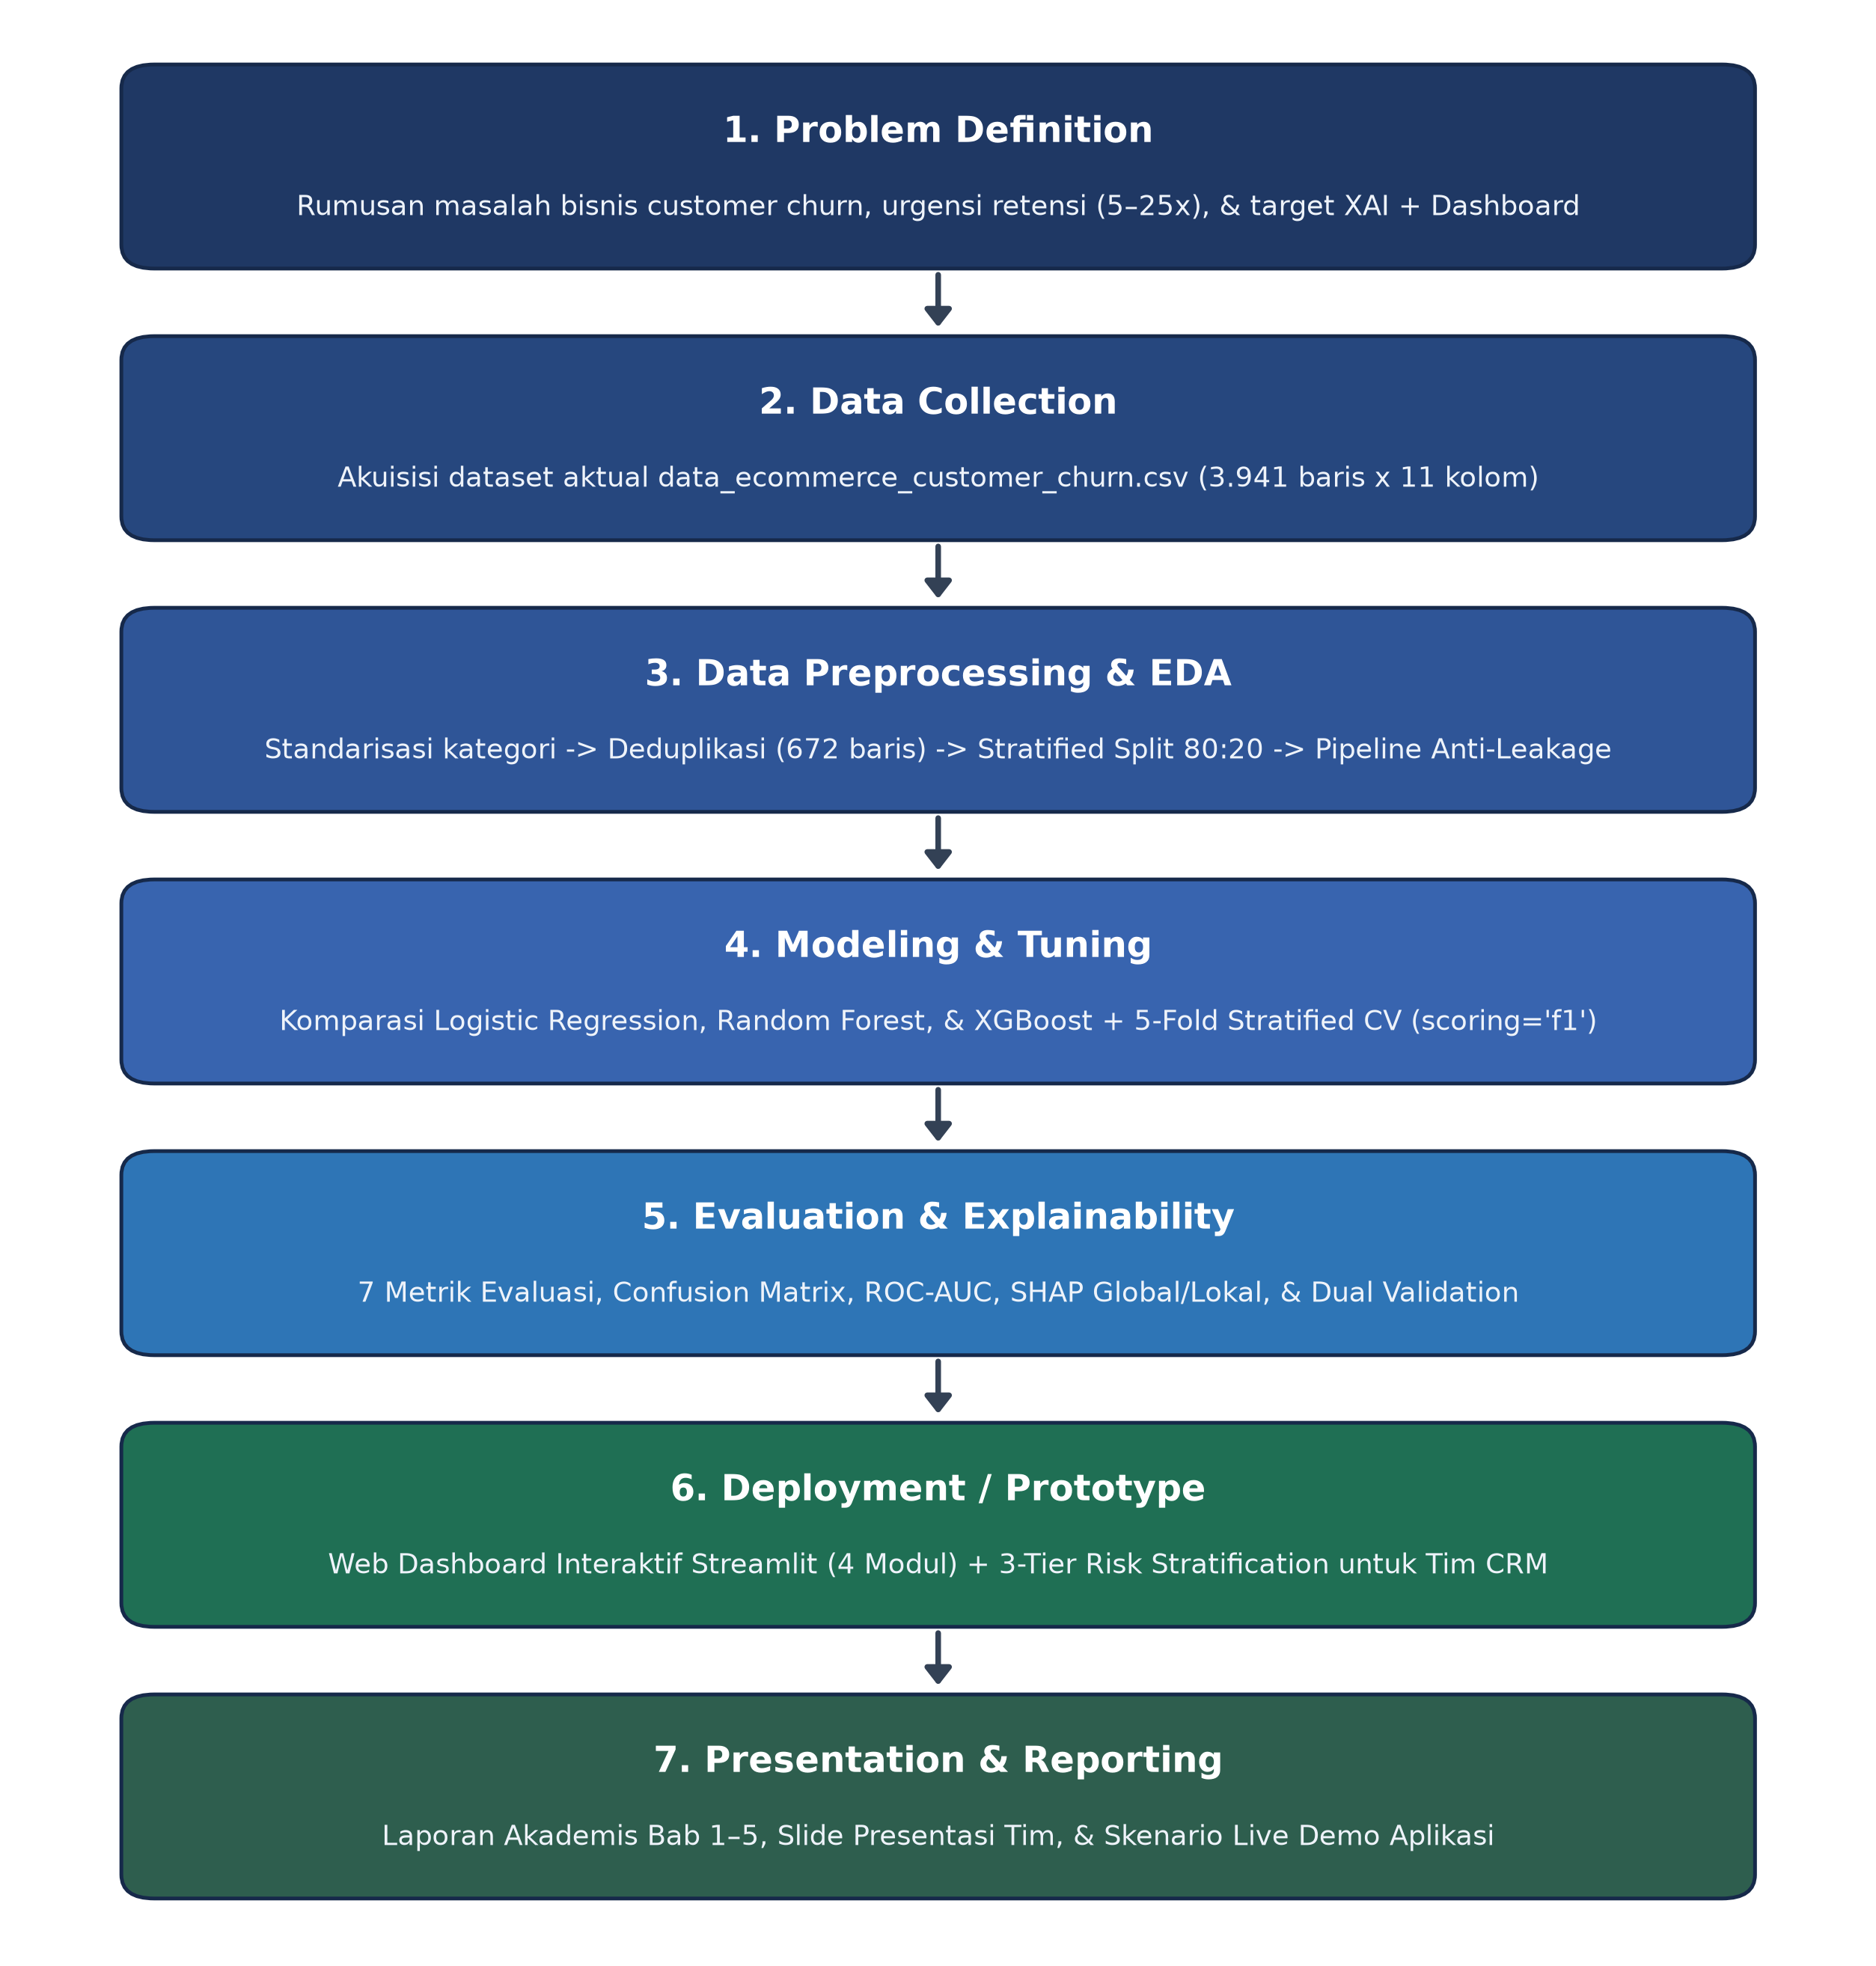
\includegraphics[width=0.92\textwidth]{gambar_3_1_alur_tbp.png}
  \caption{Alur Kerja 7 Tahapan \textit{Team-Based Project} Sistem Prediksi \textit{E-Commerce Customer Churn}}
  \label{fig:alur_tbp}
\end{figure}

\section{Manajemen Proyek, Pembagian Peran Tim, dan Alur Kolaborasi}

Sesuai prinsip \textit{Team-Based Project} yang menilai \textbf{kualitas proses kolaborasi} sekaligus \textbf{kualitas produk akhir}, pengerjaan proyek dikelola melalui pembagian peran yang jelas, kontrol versi GitHub, serta pemecahan kerja menjadi \textbf{10 Task berurutan} (\code{docs/md/tasks.md}) dengan dokumen \code{docs/md/context.md} sebagai acuan tunggal (\textit{Single Source of Truth}) seluruh anggota tim.

\begin{table}[H]
  \centering
  \caption{Matriks Pembagian Peran dan Tanggung Jawab Anggota Tim}
  \label{tab:peran_tim}
  \renewcommand{\arraystretch}{1.28}
  \setlength{\tabcolsep}{4pt}
  \footnotesize
  \begin{tabularx}{\textwidth}{@{}M{0.5cm} P{2.3cm} M{1.5cm} L P{3.7cm}@{}}
    \toprule
    \rowcolor{HeaderBlue}
    \thdr{No} & \thdr{Peran Tim} & \thdr{Anggota} & \thdr{Tanggung Jawab Utama} & \thdr{Output / Artefak} \\
    \midrule
    1 & \textbf{Leader / System Architect} & Adrian & Perancangan arsitektur repositori, koordinasi integrasi antarmodul, \textit{code review} \& \textit{merge Pull Request} di GitHub. & \code{src/config.py},\newline\code{requirements.txt},\newline\code{docs/md/*},\newline manajemen branch GitHub \\
    \rowcolor{LightRow}
    2 & \textbf{Data Engineer \& Preprocessing} & Adrian & Pemuatan data, validasi skema 11 kolom, analisis EDA \& \textit{outlier} IQR, deduplikasi, \textit{stratified split}, dan \textit{pipeline preprocessing} anti-\textit{leakage}. & \code{data\_loader.py}, \code{eda.py},\newline\code{preprocessing.py},\newline\code{data/processed/*.csv},\newline\code{eda\_summary.json} \\
    3 & \textbf{ML Modeler \& Evaluator} & Aerio & Pelatihan \& \textit{tuning} 3 model (5-Fold CV), kalkulasi 7 metrik evaluasi, integrasi SHAP (\code{TreeExplainer} \& \textit{Dual Validation}), dan mesin \textit{3-Tier Risk}. & \code{train.py}, \code{explainability.py},\newline\code{risk\_engine.py},\newline\code{models/*.joblib},\newline\code{artifacts/*.json} \\
    \rowcolor{LightRow}
    4 & \textbf{Web Prototype Developer} & Valen & Pengembangan antarmuka web interaktif berbasis Streamlit (4 modul: Individual + SHAP, \textit{Batch} CSV/Excel, Komparasi 3 Model, EDA) serta uji UI/UX. & \code{app/streamlit\_app.py},\newline\code{notebooks/\allowbreak full\_\allowbreak experiment.ipynb} \\
    5 & \textbf{Technical Writer \& Presentation} & Bombing, Daniel & Verifikasi referensi jurnal Scopus, penyusunan laporan akademis Bab 1--5, dokumentasi interpretasi bisnis SHAP, slide presentasi, \& skenario \textit{live demo}. & Laporan TBP (\code{.tex}/\code{.docx}/\code{.pdf}),\newline Slide Presentasi (\code{.pptx}),\newline\code{README.md}, koleksi referensi \\
    \bottomrule
  \end{tabularx}
\end{table}

Kolaborasi kode dikelola pada repositori GitHub (\code{aerioade/\allowbreak ecommerce-\allowbreak customer-\allowbreak churn-\allowbreak prediction}) menggunakan mekanisme \textit{feature branching} dan \textit{Pull Request} (contoh: branch \code{setup/configuration}, \code{task/data-processing}, dan \code{task/modeling-shap-risk} digabungkan ke \code{main} melalui PR \#1, PR \#2, dan PR \#3). Rencana pemecahan kerja 10 \textit{task} dirangkum pada Tabel~\ref{tab:wbs}.

\begin{table}[H]
  \centering
  \caption{Rencana Pemecahan Kerja (\textit{Work Breakdown Structure}) 10 Task Proyek}
  \label{tab:wbs}
  \renewcommand{\arraystretch}{1.28}
  \setlength{\tabcolsep}{4pt}
  \scriptsize
  \begin{tabularx}{\textwidth}{@{}M{1.0cm} L M{1.5cm} P{3.8cm} M{2.4cm}@{}}
    \toprule
    \rowcolor{HeaderBlue}
    \thdr{Task} & \thdr{Fokus Pengerjaan} & \thdr{Dependensi} & \thdr{Target Artefak} & \thdr{Tahap Pengerjaan} \\
    \midrule
    Task 1 & Setup Struktur Folder, Dependensi, \& Konfigurasi Global & --- & \code{requirements.txt},\newline\code{src/config.py} & Tahap 1 (Inisiasi \& Setup) \\
    \rowcolor{LightRow}
    Task 2 & Data Loader \& EDA (Duplikat, \textit{Missing Values}, IQR) & Task 1 & \code{data\_loader.py}, \code{eda.py},\newline\code{eda\_summary.json} & Tahap 2 (EDA \& Preprocessing) \\
    Task 3 & Preprocessing Pipeline Anti-\textit{Data Leakage} \& Split 80:20 & Task 2 & \code{preprocessing.py},\newline\code{train\_data.csv}, \code{test\_data.csv} & Tahap 2 (EDA \& Preprocessing) \\
    \rowcolor{LightRow}
    Task 4 & Pelatihan 3 Model, 5-Fold CV, \textit{Tuning}, \& Evaluasi & Task 3 & \code{train.py}, \code{models/*.joblib},\newline\code{evaluation\_metrics.json} & Tahap 3 (Modeling, SHAP, \& Risk) \\
    Task 5 & \textit{Explainable AI} (SHAP Global/Lokal) \& \textit{Dual Validation} & Task 4 & \code{explainability.py},\newline\code{feature\_importance.json} & Tahap 3 (Modeling, SHAP, \& Risk) \\
    \rowcolor{LightRow}
    Task 6 & Mesin \textit{3-Tier Risk Stratification} \& Aksi Retensi & Task 1 & \code{src/risk\_engine.py} & Tahap 3 (Modeling, SHAP, \& Risk) \\
    Task 7 & Web Dashboard: Kerangka \& Modul 1 (Individual + SHAP) & Task 5 \& 6 & \code{app/streamlit\_app.py}\newline(Modul 1) & Tahap 4 (Web Dashboard) \\
    \rowcolor{LightRow}
    Task 8 & Web Dashboard: Modul 2 (\textit{Batch Prediction} CSV/Excel) & Task 7 & \code{app/streamlit\_app.py}\newline(Modul 2) & Tahap 4 (Web Dashboard) \\
    Task 9 & Web Dashboard: Modul 3 (Komparasi) \& Modul 4 (EDA) & Task 7 & \code{app/streamlit\_app.py}\newline(Modul 3 \& 4) & Tahap 4 (Web Dashboard) \\
    \rowcolor{LightRow}
    Task 10 & Notebook Eksperimen, Laporan Akhir, Presentasi, \& Uji Akhir & Task 1--9 & \code{full\_experiment.ipynb},\newline Laporan, \code{.pptx}, Demo & Tahap 5 (Finalisasi \& Dokumentasi) \\
    \bottomrule
  \end{tabularx}
\end{table}

\section{Pengumpulan dan Spesifikasi Dataset (Tahap 2: \textit{Data Collection})}

Dataset yang digunakan adalah data sekunder publik \textit{E-Commerce Customer Churn} yang tersimpan pada \code{data/raw/\allowbreak data\_\allowbreak ecommerce\_\allowbreak customer\_\allowbreak churn.csv}. Hasil pemeriksaan awal terhadap berkas dataset aktual menunjukkan karakteristik berikut:
\begin{itemize}[leftmargin=0.8cm, itemsep=2pt]
  \item \textbf{Dimensi Data Mentah:} 3.941 baris observasi pelanggan $\times$ 11 kolom (10 fitur prediktor: 8 numerik \& 2 kategorikal, ditambah 1 target \code{Churn}).
  \item \textbf{Distribusi Target Mentah:} Kelas 0 (\textit{Non-Churn}) sebanyak 3.267 baris (82,90\%) dan kelas 1 (\textit{Churn}) sebanyak 674 baris (17,10\%), dengan rasio imbalansi $\approx$ 4,85 : 1.
  \item \textbf{Kelengkapan Data (\textit{Missing Values}):} Nilai kosong ditemukan secara alami pada tiga kolom numerik, yakni \code{DaySinceLastOrder} (213 baris / 5,40\%), \code{Tenure} (194 baris / 4,92\%), dan \code{WarehouseToHome} (169 baris / 4,29\%). Delapan kolom lainnya lengkap (0\% kosong).
  \item \textbf{Inkonsistensi Label \& Duplikasi:} Pada \code{PreferedOrderCat}, terdapat dua label bermakna sama yaitu \code{'Mobile'} (559 baris) dan \code{'Mobile Phone'} (887 baris). Selain itu, karena ketiadaan kolom \code{CustomerID}, terdapat 671 baris duplikat mentah yang menjadi \textbf{672 baris duplikat} setelah standarisasi \code{'Mobile' $\rightarrow$ 'Mobile Phone'}, menyisakan \textbf{3.269 baris unik} dengan \textbf{0 konflik label}.
\end{itemize}

\begin{table}[H]
  \centering
  \caption{Kamus Data Aktual Dataset \code{data\_ecommerce\_customer\_churn.csv} (11 Atribut)}
  \label{tab:kamus_data}
  \renewcommand{\arraystretch}{1.24}
  \setlength{\tabcolsep}{3pt}
  \scriptsize
  \begin{tabularx}{\textwidth}{@{}M{0.5cm} P{3.3cm} M{1.0cm} M{1.3cm} M{1.5cm} P{2.3cm} L@{}}
    \toprule
    \rowcolor{HeaderBlue}
    \thdr{No} & \thdr{Nama Kolom} & \thdr{Tipe} & \thdr{Peran} & \thdr{Missing (Raw)} & \thdr{Rentang / Nilai Unik Aktual} & \thdr{Deskripsi} \\
    \midrule
    1 & \code{Tenure} & float64 & Numerik & 194 (4,92\%) & 0,0--61,0 (Med: 9,0) & Lama berlangganan pada platform (bulan). \\
    \rowcolor{LightRow}
    2 & \code{WarehouseToHome} & float64 & Numerik & 169 (4,29\%) & 5,0--127,0 (Med: 14,0) & Jarak gudang pengiriman ke rumah pelanggan. \\
    3 & \code{NumberOfDeviceRegistered} & int64 & Numerik & 0 & 1--6 (Med: 4,0) & Jumlah perangkat terdaftar pada akun. \\
    \rowcolor{LightRow}
    4 & \code{PreferedOrderCat} & string & Kategorikal & 0 & Laptop \& Acc., Mobile Phone, Mobile*, Fashion, Grocery, Others & Kategori produk favorit (*\code{'Mobile'} $\rightarrow$ \code{'Mobile Phone'}). \\
    5 & \code{SatisfactionScore} & int64 & Numerik & 0 & 1--5 (Med: 3,0) & Skor kepuasan layanan pelanggan (skala 1--5). \\
    \rowcolor{LightRow}
    6 & \code{MaritalStatus} & string & Kategorikal & 0 & Married, Single, Divorced & Status pernikahan pelanggan. \\
    7 & \code{NumberOfAddress} & int64 & Numerik & 0 & 1--22 (Med: 3,0) & Jumlah alamat pengiriman terdaftar. \\
    \rowcolor{LightRow}
    8 & \code{Complain} & int64 & Biner & 0 & 0 (Tidak), 1 (Ya) & Riwayat mengajukan komplain bulan terakhir. \\
    9 & \code{DaySinceLastOrder} & float64 & Numerik & 213 (5,40\%) & 0,0--46,0 (Med: 3,0) & Jarak hari sejak pesanan terakhir. \\
    \rowcolor{LightRow}
    10 & \code{CashbackAmount} & float64 & Numerik & 0 & 0,0--324,99 (Med: 163,34) & Rata-rata nilai \textit{cashback} yang diterima. \\
    11 & \code{Churn} & int64 & \textbf{Target} & 0 & 0 (Non-Churn), 1 (Churn) & Status retensi pelanggan (0 = Bertahan, 1 = Churn). \\
    \bottomrule
  \end{tabularx}
\end{table}

\section{Rancangan Preprocessing Anti-\textit{Data Leakage} dan Seleksi Atribut (Tahap 3)}

Untuk mencegah kebocoran informasi dari data uji ke data latih (\textit{data leakage}), seluruh tahapan penyiapan data dijalankan dengan urutan eksekusi ketat sebagaimana ditunjukkan pada Gambar~\ref{fig:anti_leakage}.

\begin{figure}[H]
  \centering
  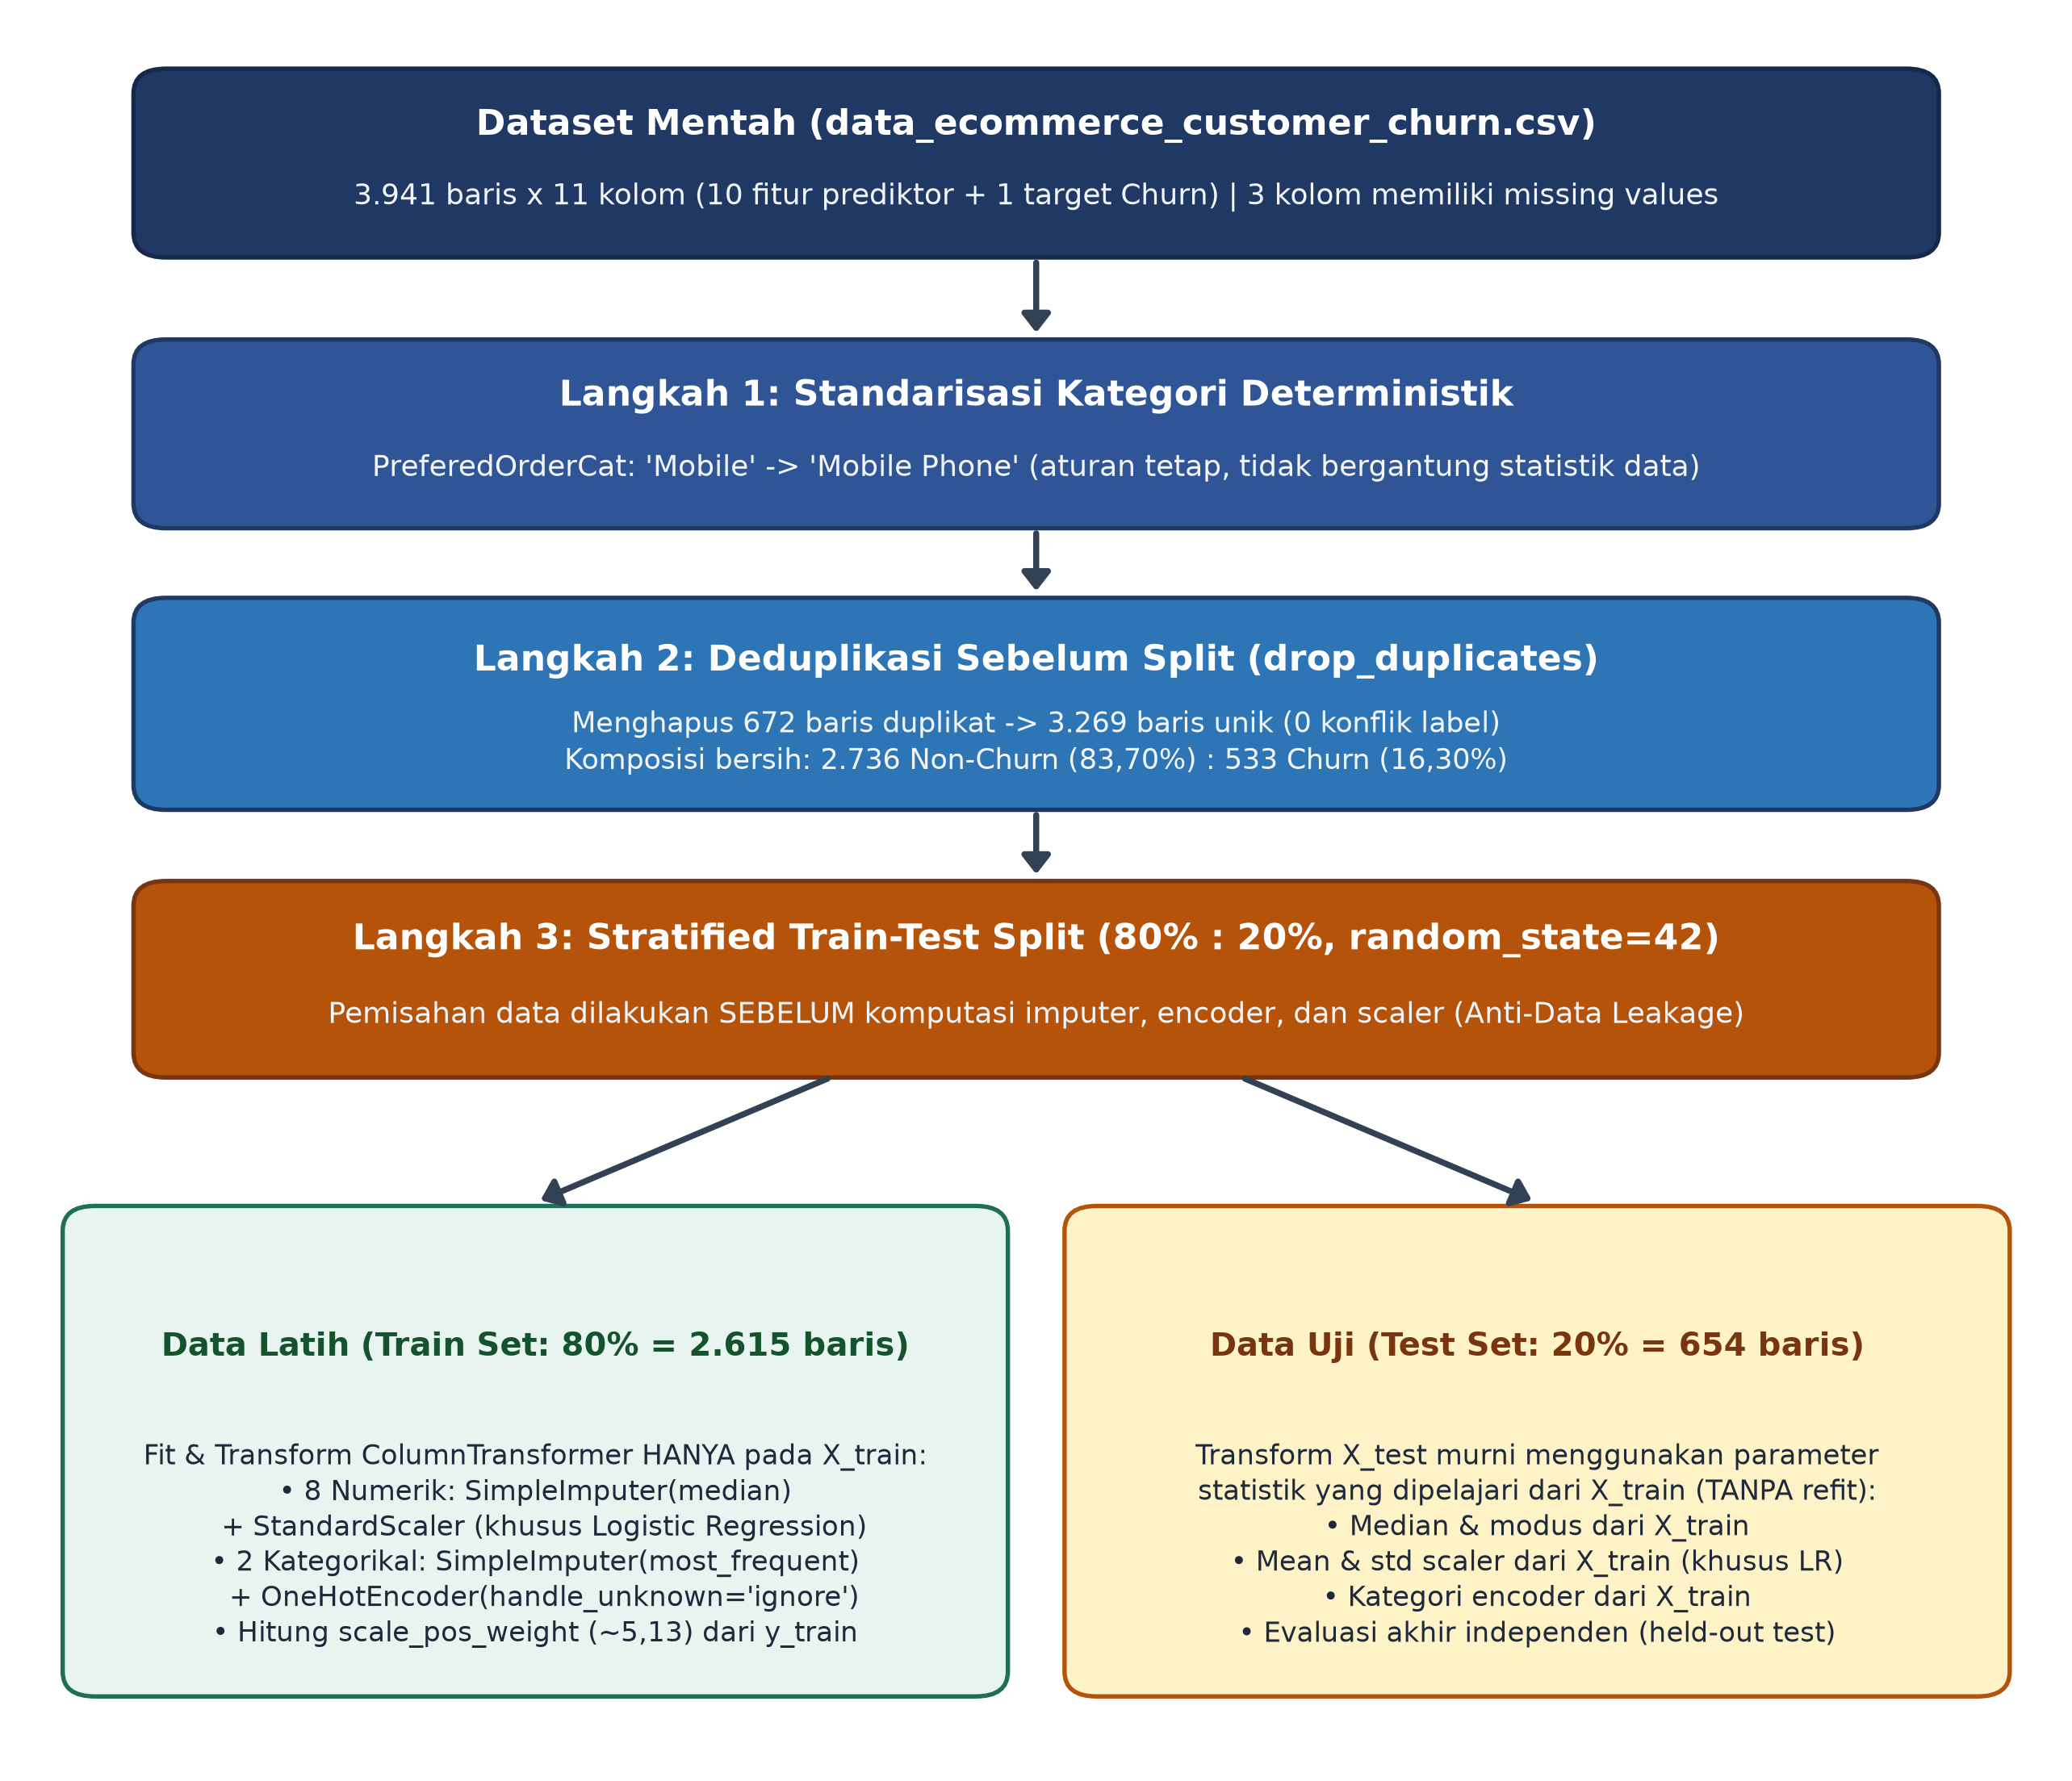
\includegraphics[width=0.95\textwidth]{gambar_3_2_anti_leakage.png}
  \caption{Protokol \textit{Data Preprocessing} Anti-\textit{Data Leakage}}
  \label{fig:anti_leakage}
\end{figure}

\begin{enumerate}[leftmargin=0.8cm, itemsep=2pt]
  \item \textbf{Standarisasi Kategori Deterministik (\code{src/data\_loader.py}):} Pemetaan \code{'Mobile' $\rightarrow$ 'Mobile Phone'} pada \code{PreferedOrderCat} bersifat deterministik (tidak bergantung pada statistik data) sehingga aman diterapkan sebelum pemisahan data.
  \item \textbf{Deduplikasi Sebelum Split:} Penghapusan \textbf{672 baris duplikat} dilakukan sebelum \code{train\_test\_split} agar sampel identik tidak bocor ke partisi latih dan uji bersamaan. Diperoleh \textbf{3.269 baris unik} dengan komposisi \textbf{2.736 Non-Churn (83,70\%)} dan \textbf{533 Churn (16,30\%)} (rasio imbalansi $\approx$ 5,13 : 1).
  \item \textbf{Stratified Train-Test Split (80:20):} Data bersih dibagi secara berstrata (\code{stratify=y, random\_state=42}) menjadi \textbf{2.615 baris data latih} (\code{train\_data.csv}) dan \textbf{654 baris data uji} (\code{test\_data.csv}) sebelum komputasi imputasi, \textit{encoding}, atau \textit{scaling} apa pun.
  \item \textbf{Transformasi Fitur di Dalam \code{ColumnTransformer} \& \code{Pipeline}:} Kedelapan fitur numerik diimputasi dengan \code{SimpleImputer(strategy='median')} (lebih tahan terhadap \textit{outlier}), ditambah \code{StandardScaler()} khusus pada \textit{pipeline} Logistic Regression. Dua fitur kategorikal diimputasi dengan \code{most\_frequent} lalu dikodekan dengan \code{OneHotEncoder(handle\_unknown='ignore', sparse\_output=False)} yang mendukung \code{get\_feature\_names\_out()} demi pemetaan nama fitur SHAP.
  \item \textbf{Dokumentasi Outlier IQR Tanpa Penghapusan:} \textit{Outlier} pada 6 fitur numerik kontinu dideteksi menggunakan Persamaan~\eqref{eq:iqr}--\eqref{eq:ub} dan dicatat pada \code{artifacts/eda\_summary.json}, namun tidak dihapus karena merepresentasikan keragaman perilaku pelanggan nyata dan ditangani dengan baik oleh model berbasis pohon.
  \item \textbf{Pertimbangan Seleksi Atribut dan Keputusan Tanpa PCA:} Seluruh 10 fitur perilaku dan demografi aktual dipertahankan karena tidak terdapat kolom ID non-prediktif maupun redundansi ekstrem yang harus dibuang manual. Reduksi dimensi PCA \textbf{tidak diterapkan} agar nama fitur asli tetap utuh dan mudah dipahami pada visualisasi SHAP. Pemeringkatan serta validasi relevansi setiap atribut dilakukan secara kuantitatif melalui \textbf{Global SHAP Importance} dan \textbf{Tree Feature Importance}.
\end{enumerate}

\section{Rancangan Pemodelan, \textit{Tuning}, dan Evaluasi (Tahap 4 \& 5)}

Ketiga algoritma dibungkus dalam objek \code{Pipeline} (\code{preprocessor + classifier}) dan dioptimasi pada data latih menggunakan \code{StratifiedKFold(n\_splits=5, shuffle=True, random\_state=42)} dengan metrik optimasi utama \code{scoring='f1'}. Konfigurasi dasar dan ruang pencarian \textit{hyperparameter} dirangkum pada Tabel~\ref{tab:tuning}.

\begin{table}[H]
  \centering
  \caption{Konfigurasi Dasar dan Ruang \textit{Hyperparameter Tuning} Tiga Algoritma}
  \label{tab:tuning}
  \renewcommand{\arraystretch}{1.28}
  \setlength{\tabcolsep}{3.5pt}
  \scriptsize
  \begin{tabularx}{\textwidth}{@{}P{1.9cm} M{1.6cm} M{2.4cm} P{3.2cm} L@{}}
    \toprule
    \rowcolor{HeaderBlue}
    \thdr{Algoritma} & \thdr{Paradigma} & \thdr{Penanganan Imbalance} & \thdr{Pengaturan Dasar} & \thdr{Ruang Pencarian \textit{Hyperparameter}} \\
    \midrule
    \textbf{Logistic Regression} & Linear Baseline & \code{class\_weight=}\newline\code{'balanced'} & \code{max\_iter=1000}\newline\code{random\_state=42}\newline StandardScaler aktif & \code{C}: [0.01, 0.1, 1.0, 10.0]\newline\code{solver}: ['lbfgs'] \\
    \rowcolor{LightRow}
    \textbf{Random Forest} & Ensemble Bagging & \code{class\_weight=}\newline\code{'balanced'} & \code{random\_state=42}\newline\code{n\_jobs=-1}\newline tanpa \textit{scaling} & \code{n\_estimators}: [100, 200, 300]\newline\code{max\_depth}: [None, 10, 20, 30]\newline\code{min\_samples\_split}: [2, 5, 10]\newline\code{min\_samples\_leaf}: [1, 2, 4] \\
    \textbf{XGBoost} & Ensemble Boosting & \code{scale\_pos\_weight}\newline($\approx 5{,}13$ dari \code{y\_train}) & \code{eval\_metric='logloss'}\newline\code{random\_state=42}\newline\code{n\_jobs=-1}\newline tanpa \textit{scaling} & \code{n\_estimators}: [100, 200, 300]\newline\code{max\_depth}: [3, 5, 7, 9]\newline\code{learning\_rate}: [0.01, 0.05, 0.1, 0.2]\newline\code{subsample}: [0.8, 1.0]\newline\code{colsample\_bytree}: [0.8, 1.0] \\
    \bottomrule
  \end{tabularx}
\end{table}

Ketiga model hasil \textit{tuning} dievaluasi secara objektif pada \textit{held-out test set} (654 baris) menggunakan seluruh tujuh metrik pada Persamaan~\eqref{eq:acc}--\eqref{eq:auc}. Model terbaik dipilih berdasarkan nilai \textbf{F1-Score tertinggi} (dengan \textbf{ROC-AUC} sebagai penentu jika seri) lalu diserialisasi ke \code{models/best\_model\_pipeline.joblib}. Pada tahap interpretabilitas (\code{src/explainability.py}), \code{TreeExplainer} digunakan untuk menghitung kontribusi SHAP global dan lokal (menangani output 2D pada XGBoost serta irisan kelas positif pada output 3D Random Forest), diikuti \textbf{Dual Validation} terhadap \code{feature\_importances\_} bawaan model yang disimpan di \code{artifacts/feature\_importance.json}.

\section{Rancangan \textit{Prototype Web Dashboard} dan Strategi Retensi (Tahap 6)}

Untuk menghasilkan produk solusi nyata (\textit{product-centered TBP}), model terlatih, modul SHAP, dan mesin aturan risiko (\code{src/risk\_engine.py}) diintegrasikan ke dalam aplikasi web interaktif berbasis \textbf{Streamlit} (\code{app/streamlit\_app.py}) yang terdiri atas empat modul fungsional:
\begin{enumerate}[leftmargin=0.8cm, itemsep=2pt]
  \item \textbf{Modul 1 --- Prediksi Individual \& Penjelasan SHAP Lokal:} Form input interaktif 10 fitur pelanggan, output probabilitas \textit{churn} (\%), status prediksi, \textit{badge Risk Tier}, kotak rekomendasi retensi otomatis, \textbf{SHAP Waterfall Plot}, serta ringkasan Top 3 faktor pendorong dan Top 3 penahan risiko.
  \item \textbf{Modul 2 --- \textit{Batch Prediction} (Unggah CSV / Excel):} Unduh \textit{template} CSV 10 kolom, validasi skema \& standarisasi otomatis, KPI ringkasan \textit{batch}, grafik distribusi \textit{Risk Tier}, tabel hasil, dan tombol unduh CSV hasil prediksi.
  \item \textbf{Modul 3 --- Dashboard Analitik \& Komparasi 3 Model:} Tabel metrik evaluasi berdampingan, \textit{Grouped Bar Chart}, kurva \textit{ROC-AUC} gabungan, \textit{Confusion Matrix} interaktif per model, dan grafik \textbf{Validasi Ganda} (\textit{Global SHAP} vs \textit{Tree Gain/Gini Importance}).
  \item \textbf{Modul 4 --- Eksplorasi Data (EDA) \& Ringkasan Proyek:} Statistik pembersihan data (3.941 $\rightarrow$ 3.269 baris unik), grafik tingkat \textit{churn} per kategori, tabel deteksi \textit{outlier} IQR, serta ringkasan metodologi anti-\textit{data leakage} dan referensi ilmiah.
\end{enumerate}

Pemetaan probabilitas prediksi $p = P(y = 1 \mid \mathbf{x})$ menuju rekomendasi aksi operasional tim CRM ditetapkan melalui aturan \textbf{\textit{3-Tier Risk Stratification}} pada Tabel~\ref{tab:risk_tier}.

\begin{table}[H]
  \centering
  \caption{Aturan \textit{3-Tier Risk Stratification} dan Rekomendasi Aksi Retensi Otomatis}
  \label{tab:risk_tier}
  \renewcommand{\arraystretch}{1.28}
  \setlength{\tabcolsep}{4pt}
  \footnotesize
  \begin{tabularx}{\textwidth}{@{}M{1.7cm} M{2.1cm} M{1.7cm} L L@{}}
    \toprule
    \rowcolor{HeaderBlue}
    \thdr{Tingkat Risiko} & \thdr{Ambang ($p$)} & \thdr{Warna UI} & \thdr{Indikasi Perilaku Utama} & \thdr{Rekomendasi Aksi Retensi Otomatis (Tim CRM)} \\
    \midrule
    \textbf{High Risk} & $p \ge 0{,}65$ & \textbf{Merah}\newline(\code{\#DC2626}) & Risiko \textit{churn} sangat tinggi (ada riwayat komplain, masa langganan baru, skor kepuasan rendah). & \textbf{Prioritas \textit{Service Recovery}:} Hubungi pelanggan proaktif via CS/CRM dalam 24 jam, selesaikan keluhan, \& berikan voucher retensi personal. \\
    \rowcolor{LightRow}
    \textbf{Medium Risk} & $0{,}35 \le p < 0{,}65$ & \textbf{Oranye}\newline(\code{\#D97706}) & Keterlibatan (\textit{engagement}) mulai menurun atau jeda dari transaksi terakhir semakin panjang. & \textbf{Kampanye \textit{Re-Engagement}:} Kirim notifikasi personalisasi sesuai kategori favorit, promo \textit{cashback} terarah, atau pengingat kupon aktif. \\
    \textbf{Low Risk} & $p < 0{,}35$ & \textbf{Hijau}\newline(\code{\#16A34A}) & Pelanggan loyal, transaksi rutin terjaga, dan tingkat kepuasan baik. & \textbf{\textit{Loyalty Reinforcement}:} Pertahankan loyalitas lewat program poin / VIP \textit{tier} dan \textit{early access} produk baru tanpa diskon agresif. \\
    \bottomrule
  \end{tabularx}
\end{table}

% ============================================================
% BAB 4: HASIL, IMPLEMENTASI, DAN PEMBAHASAN
% ============================================================
\chapter{Hasil, Implementasi, dan Pembahasan}

\section{Hasil Eksplorasi Data (EDA), Deduplikasi, dan Deteksi Outlier IQR}

Tahap eksplorasi data (\textit{Exploratory Data Analysis}) dan pembersihan awal dijalankan melalui modul \code{src/data\_loader.py} dan \code{src/eda.py} yang menghasilkan ringkasan terstruktur pada \code{artifacts/eda\_summary.json}. Dari total \textbf{3.941 baris mentah} dan \textbf{11 kolom}, dilakukan standarisasi kategori deterministik pada atribut \code{PreferedOrderCat} (\code{'Mobile' $\rightarrow$ 'Mobile Phone'}) yang disusul oleh penghapusan baris duplikat (\code{drop\_duplicates()}) sebelum pemisahan data. Standarisasi tersebut mengungkap 1 pasangan baris tambahan yang identik, sehingga total \textbf{672 baris duplikat} (bertambah dari 671 duplikat mentah) berhasil dieliminasi dan menyisakan \textbf{3.269 baris pelanggan unik}.

Pada dataset bersih (\textbf{3.269 baris}), kelas \textbf{Non-Churn (0)} berjumlah \textbf{2.736 baris (83,70\%)} sedangkan kelas \textbf{Churn (1)} berjumlah \textbf{533 baris (16,30\%)}, dengan rasio imbalansi \textbf{5,13 : 1}. Selanjutnya, partisi \textit{Stratified Train-Test Split (80:20)} melalui \code{src/preprocessing.py} menghasilkan \textbf{2.615 baris data latih} (\code{train\_data.csv}: 2.189 Non-Churn [83,71\%] dan 426 Churn [16,29\%]) serta \textbf{654 baris data uji} (\code{test\_data.csv}: 547 Non-Churn [83,64\%] dan 107 Churn [16,36\%]). Proporsi kelas target terjaga identik pada kedua partisi, dan nilai \code{scale\_pos\_weight} untuk model XGBoost dihitung secara eksklusif dari \code{y\_train} sebesar \textbf{5,1385} ($2.189 / 426$). Ringkasan pembersihan dan partisi data disajikan pada Tabel~\ref{tab:partisi}.

\begin{table}[H]
  \centering
  \caption{Ringkasan Pembersihan Data, Distribusi Kelas Target, dan Partisi \textit{Train-Test Split}}
  \label{tab:partisi}
  \renewcommand{\arraystretch}{1.28}
  \setlength{\tabcolsep}{3.5pt}
  \scriptsize
  \begin{tabularx}{\textwidth}{@{}P{2.4cm} M{1.1cm} M{2.0cm} M{1.9cm} M{1.3cm} L@{}}
    \toprule
    \rowcolor{HeaderBlue}
    \thdr{Tahap / Partisi Data} & \thdr{Total Baris} & \thdr{Non-Churn (0)} & \thdr{Churn (1)} & \thdr{Rasio (0:1)} & \thdr{Keterangan Teknis} \\
    \midrule
    Dataset Mentah (Raw) & 3.941 & 3.267 (82,90\%) & 674 (17,10\%) & 4,85 : 1 & Terdapat 671 duplikat mentah; \textit{missing} pada 3 fitur numerik. \\
    \rowcolor{LightRow}
    Setelah Standarisasi \& Deduplikasi & 3.269 & 2.736 (83,70\%) & 533 (16,30\%) & 5,13 : 1 & 672 duplikat dihapus (\code{'Mobile'} $\rightarrow$ \code{'Mobile Phone'}); 0 konflik label. \\
    Data Latih (Train Set 80\%) & 2.615 & 2.189 (83,71\%) & 426 (16,29\%) & 5,14 : 1 & Dipakai untuk \textit{fit} \code{ColumnTransformer} \& 5-Fold CV (\code{scale\_pos\_weight} = 5,1385). \\
    \rowcolor{LightRow}
    Data Uji (Test Set 20\%) & 654 & 547 (83,64\%) & 107 (16,36\%) & 5,11 : 1 & \textit{Held-out test set} independen (transformasi memakai parameter Train). \\
    \bottomrule
  \end{tabularx}
\end{table}

Adapun nilai kosong (\textit{missing values}) pada dataset bersih tercatat pada tiga fitur numerik kontinu, yaitu \code{DaySinceLastOrder} (181 baris / 5,54\%), \code{Tenure} (159 baris / 4,86\%), dan \code{WarehouseToHome} (135 baris / 4,13\%). Ketiga kolom tersebut diimputasi menggunakan median data latih di dalam \code{ColumnTransformer}. Sementara itu, hasil statistik deskriptif serta deteksi \textit{outlier} metode \textit{Interquartile Range} (IQR) pada enam fitur numerik kontinu dataset bersih dirangkum pada Tabel~\ref{tab:iqr}.

\begin{table}[H]
  \centering
  \caption{Statistik Deskriptif dan Deteksi \textit{Outlier} Metode IQR pada Dataset Bersih ($n = 3.269$)}
  \label{tab:iqr}
  \renewcommand{\arraystretch}{1.28}
  \setlength{\tabcolsep}{3.5pt}
  \scriptsize
  \begin{tabularx}{\textwidth}{@{}P{3.6cm} C C C C C@{}}
    \toprule
    \rowcolor{HeaderBlue}
    \thdr{Fitur Numerik} & \thdr{Mean / Median} & \thdr{$Q_1$; $Q_3$} & \thdr{Batas IQR [LB; UB]} & \thdr{Rentang [Min--Max]} & \thdr{Jumlah Outlier (\%)} \\
    \midrule
    \code{Tenure} & 10,19 / 9,00 & [2,00; 16,00] & [-19,00; 37,00] & 0,00--61,00 & 4 (0,13\%) \\
    \rowcolor{LightRow}
    \code{WarehouseToHome} & 15,51 / 13,00 & [9,00; 20,00] & [-7,50; 36,50] & 5,00--127,00 & 1 (0,03\%) \\
    \code{NumberOfDeviceRegistered} & 3,68 / 4,00 & [3,00; 4,00] & [1,50; 5,50] & 1,00--6,00 & 226 (6,91\%) \\
    \rowcolor{LightRow}
    \code{NumberOfAddress} & 4,22 / 3,00 & [2,00; 6,00] & [-4,00; 12,00] & 1,00--22,00 & 3 (0,09\%) \\
    \code{DaySinceLastOrder} & 4,55 / 3,00 & [2,00; 7,00] & [-5,50; 14,50] & 0,00--46,00 & 40 (1,30\%) \\
    \rowcolor{LightRow}
    \code{CashbackAmount} & 177,44 / 163,89 & [145,90; 197,14] & [69,04; 274,00] & 0,00--324,99 & 253 (7,74\%) \\
    \bottomrule
  \end{tabularx}
\end{table}

Berdasarkan Tabel~\ref{tab:iqr}, proporsi \textit{outlier} tertinggi secara matematis terjadi pada \code{CashbackAmount} (253 baris / 7,74\%, sebagian besar penerima \textit{cashback} tinggi hingga 324,99) dan \code{NumberOfDeviceRegistered} (226 baris / 6,91\%, yang terdeteksi akibat sifat diskrit integer dengan $Q_1 = 3$ dan $Q_3 = 4$). Pada \code{WarehouseToHome} ditemukan 1 nilai ekstrem jarak pengiriman sejauh 127,0 serta 40 observasi pada \code{DaySinceLastOrder} dengan jeda hingga 46 hari. Seluruh \textit{outlier} tetap dipertahankan sesuai aturan proyek karena merepresentasikan variasi transaksi nyata.

Selanjutnya, analisis tingkat \textit{churn} per kategori pada fitur \code{PreferedOrderCat} dan \code{MaritalStatus} (Tabel~\ref{tab:churn_cat} dan Gambar~\ref{fig:eda_kategori}) memperlihatkan perbedaan kerentanan yang tajam antarsegmen pelanggan.

\begin{table}[H]
  \centering
  \caption{Distribusi Tingkat Churn (\textit{Churn Rate}) Berdasarkan Fitur Kategorikal ($n = 3.269$)}
  \label{tab:churn_cat}
  \renewcommand{\arraystretch}{1.28}
  \setlength{\tabcolsep}{4pt}
  \footnotesize
  \begin{tabularx}{\textwidth}{@{}P{2.8cm} P{2.7cm} C C C C@{}}
    \toprule
    \rowcolor{HeaderBlue}
    \thdr{Atribut} & \thdr{Kategori} & \thdr{Total Pelanggan} & \thdr{Non-Churn (0)} & \thdr{Churn (1)} & \thdr{Churn Rate (\%)} \\
    \midrule
    \code{PreferedOrderCat} & Mobile Phone & 1.182 & 864 & 318 & \textbf{26,90\%} \\
    \rowcolor{LightRow}
    \code{PreferedOrderCat} & Fashion & 484 & 409 & 75 & 15,50\% \\
    \code{PreferedOrderCat} & Laptop \& Accessory & 1.213 & 1.094 & 119 & 9,81\% \\
    \rowcolor{LightRow}
    \code{PreferedOrderCat} & Others & 149 & 138 & 11 & 7,38\% \\
    \code{PreferedOrderCat} & Grocery & 241 & 231 & 10 & 4,15\% \\
    \rowcolor{LightRow}
    \code{MaritalStatus} & Single & 1.007 & 747 & 260 & \textbf{25,82\%} \\
    \code{MaritalStatus} & Divorced & 576 & 487 & 89 & 15,45\% \\
    \rowcolor{LightRow}
    \code{MaritalStatus} & Married & 1.686 & 1.502 & 184 & 10,91\% \\
    \bottomrule
  \end{tabularx}
\end{table}

\begin{figure}[H]
  \centering
  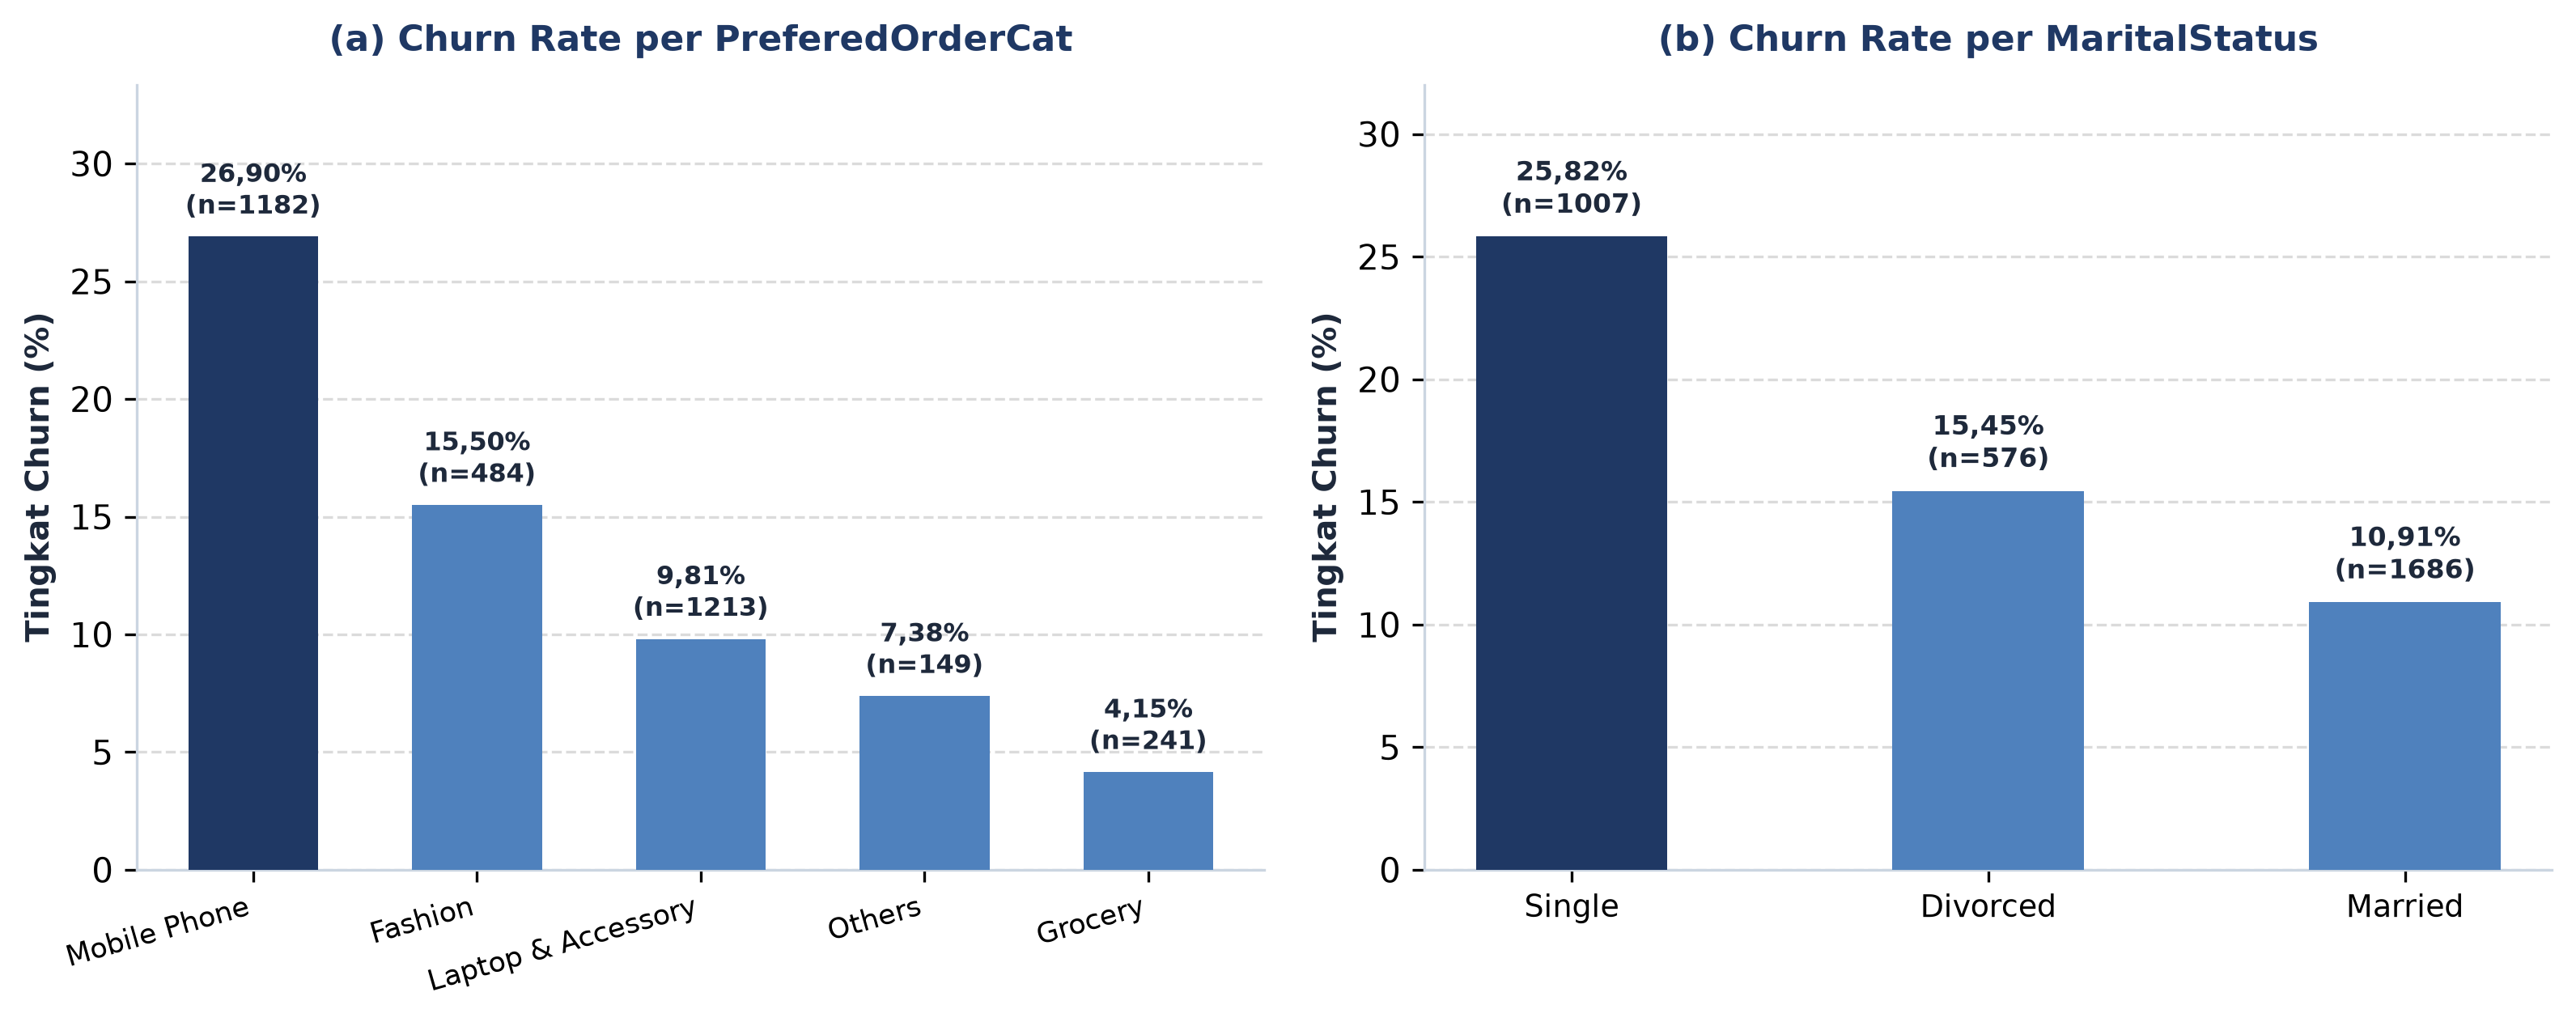
\includegraphics[width=\textwidth]{gambar_4_1_eda_kategori.png}
  \caption{Tingkat Churn (\textit{Churn Rate}) per Kategori \code{PreferedOrderCat} dan \code{MaritalStatus}}
  \label{fig:eda_kategori}
\end{figure}

Pada atribut \code{PreferedOrderCat}, pembeli kategori \textbf{Mobile Phone} memiliki risiko \textit{churn} tertinggi sebesar \textbf{26,90\%} (318 dari 1.182 pelanggan), hampir dua kali lipat dari rata-rata keseluruhan (16,30\%) dan enam kali lebih tinggi dibandingkan segmen \textbf{Grocery} (4,15\%) yang cenderung berbelanja kebutuhan pokok secara rutin. Pada atribut \code{MaritalStatus}, pelanggan berstatus \textbf{Single} mencatat tingkat \textit{churn} tertinggi sebesar \textbf{25,82\%}, lebih dari dua kali lipat dibandingkan pelanggan \textbf{Married} (10,91\%), yang mengindikasikan loyalitas transaksi rumah tangga cenderung lebih stabil.

\section{Hasil Pelatihan, \textit{Hyperparameter Tuning}, dan Komparasi Tiga Model Klasifikasi}

Pelatihan dan optimasi ketiga algoritma (\textbf{Logistic Regression}, \textbf{Random Forest}, dan \textbf{XGBoost}) dijalankan melalui modul \code{src/train.py} pada 2.615 data latih menggunakan \textit{5-Fold Stratified Cross-Validation} dengan metrik optimasi \code{scoring='f1'}. Hasil konfigurasi \textit{hyperparameter} terbaik beserta evaluasi lengkap pada \textit{held-out test set} (654 baris) dirangkum pada Tabel~\ref{tab:evaluasi}.

\begin{table}[H]
  \centering
  \caption{Hasil \textit{Hyperparameter Tuning} dan Perbandingan Kinerja Tiga Model pada \textit{Test Set} ($n = 654$)}
  \label{tab:evaluasi}
  \renewcommand{\arraystretch}{1.28}
  \setlength{\tabcolsep}{4pt}
  \footnotesize
  \begin{tabularx}{\textwidth}{@{}P{3.3cm} C C C@{}}
    \toprule
    \rowcolor{HeaderBlue}
    \thdr{Metrik / Parameter} & \thdr{Logistic Regression (\textit{Linear Baseline})} & \thdr{Random Forest (\textit{Ensemble Bagging})} & \thdr{XGBoost (\textit{Boosting} --- Terbaik)} \\
    \midrule
    \textbf{Hyperparameter Terbaik} & {\scriptsize\code{C=10,0}\newline\code{solver='lbfgs'}} & {\scriptsize\code{n\_estimators=300}\newline\code{max\_depth=30}\newline\code{min\_samples\_split=2}\newline\code{min\_samples\_leaf=1}} & {\scriptsize\code{n\_estimators=300}\newline\code{max\_depth=7}\newline\code{learning\_rate=0,05}\newline\code{subsample=0,8}\newline\code{colsample\_bytree=1,0}} \\
    \rowcolor{LightRow}
    \textbf{Mean CV F1-Score (5-Fold)} & 54,66\% & 73,96\% & 73,63\% \\
    \textbf{Confusion Matrix (TN/FP/FN/TP)} & 419 / 128 / 10 / 97 & 512 / 35 / 16 / 91 & \textbf{517 / 30 / 15 / 92} \\
    \rowcolor{LightRow}
    \textbf{Accuracy} & 78,90\% & 92,20\% & \textbf{93,12\%} \\
    \textbf{Precision} & 43,11\% & 72,22\% & \textbf{75,41\%} \\
    \rowcolor{LightRow}
    \textbf{Recall (Sensitivity)} & \textbf{90,65\%} & 85,05\% & 85,98\% \\
    \textbf{Specificity (TNR)} & 76,60\% & 93,60\% & \textbf{94,52\%} \\
    \rowcolor{LightRow}
    \textbf{False Positive Rate (FPR)} & 23,40\% & 6,40\% & \textbf{5,48\%} \\
    \rowcolor{HighlightRow}
    \textbf{F1-Score (Metrik Utama)} & 58,43\% & 78,11\% & \textbf{80,35\%} \\
    \textbf{ROC-AUC} & 0,9194 & 0,9636 & \textbf{0,9665} \\
    \bottomrule
  \end{tabularx}
\end{table}

\begin{figure}[H]
  \centering
  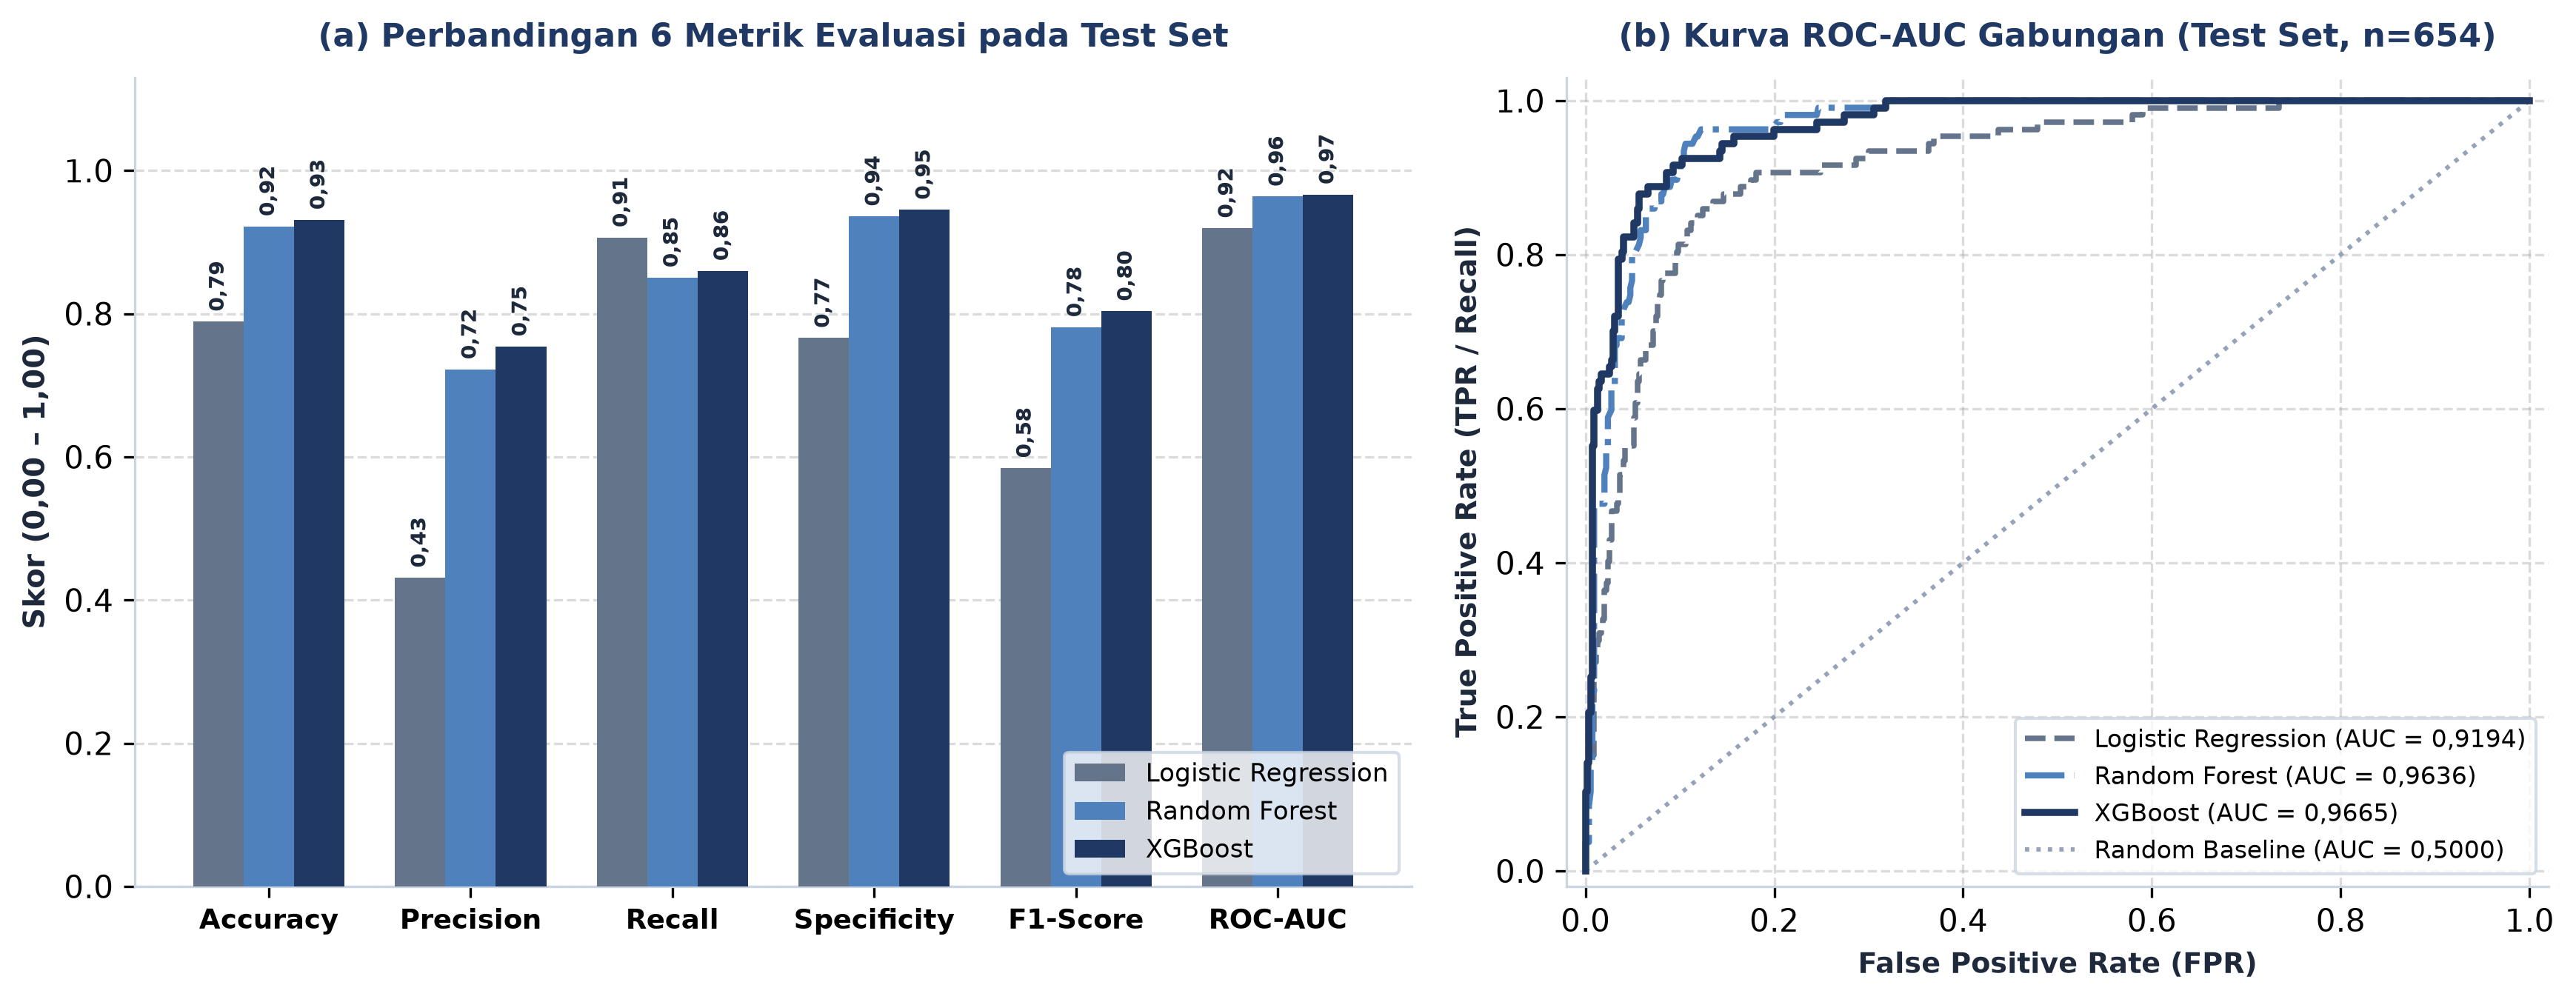
\includegraphics[width=\textwidth]{gambar_4_2_komparasi_roc.png}
  \caption{Perbandingan Enam Metrik Evaluasi dan Kurva ROC-AUC Ketiga Algoritma pada \textit{Test Set}}
  \label{fig:komparasi_roc}
\end{figure}

\begin{figure}[H]
  \centering
  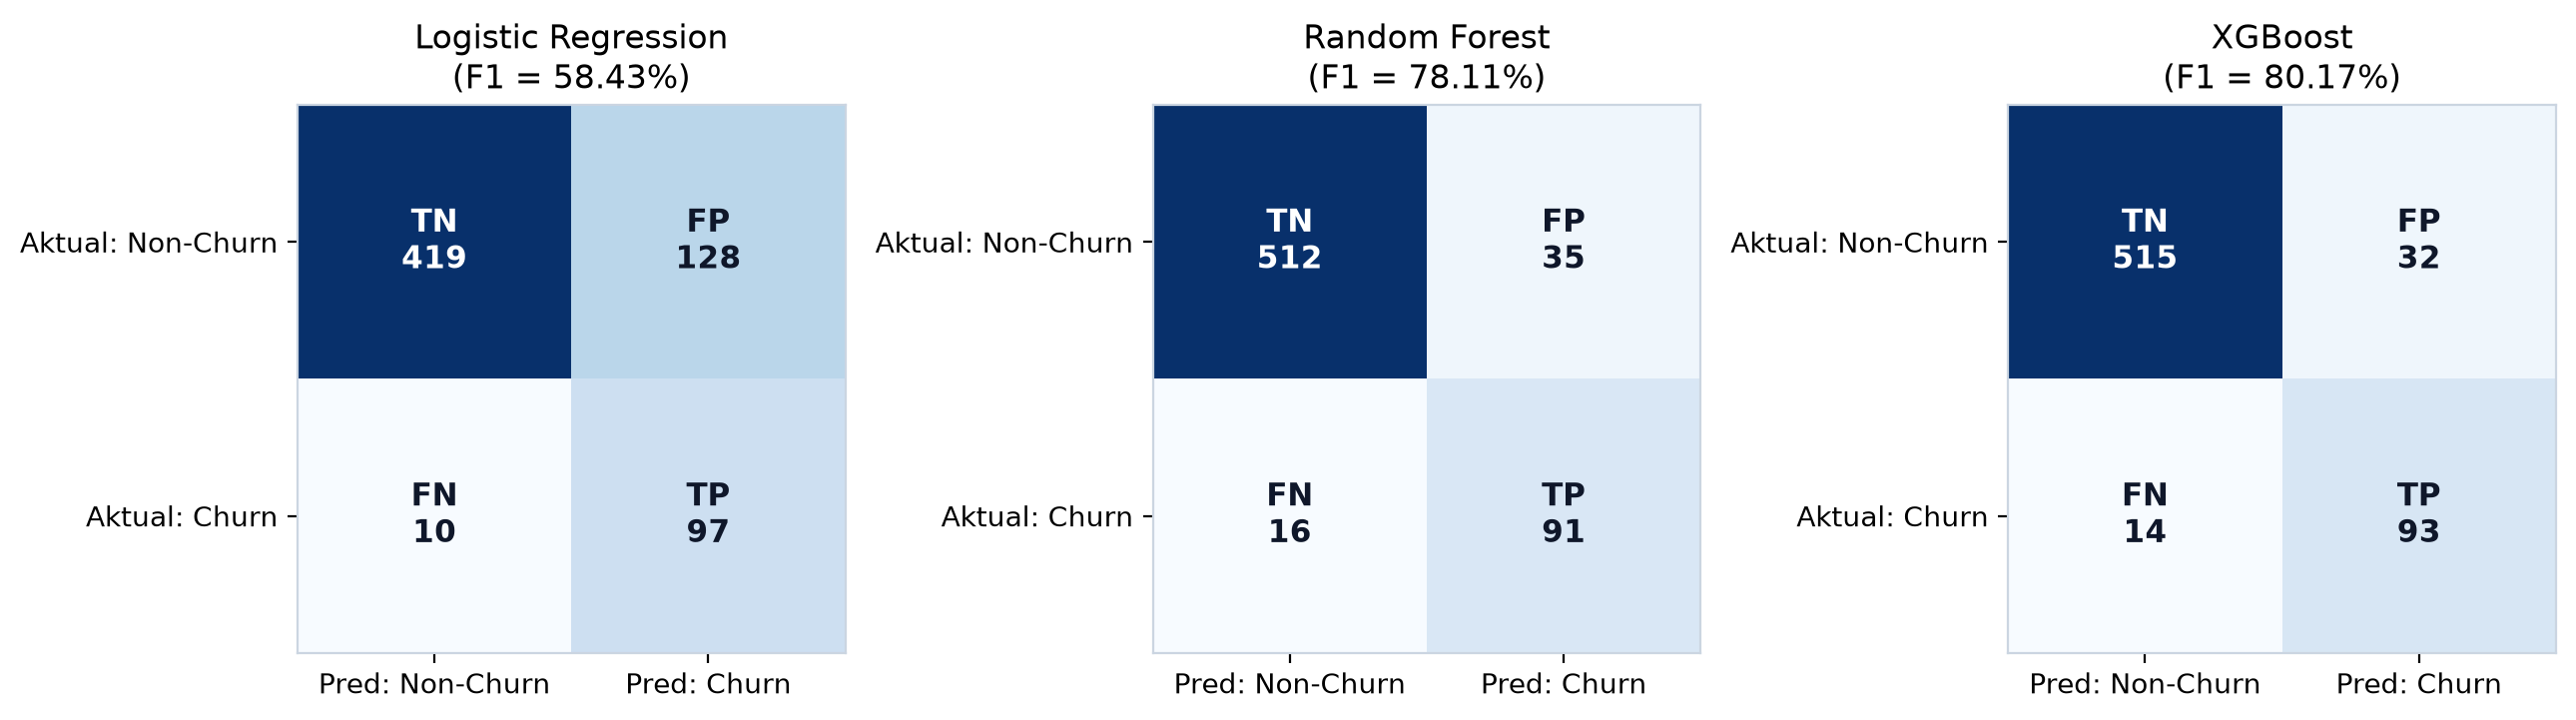
\includegraphics[width=\textwidth]{gambar_4_3_confusion_matrix.png}
  \caption{\textit{Confusion Matrix} Ketiga Model Klasifikasi pada \textit{Test Set} ($n = 654$)}
  \label{fig:cm}
\end{figure}

Hasil komparasi pada Tabel~\ref{tab:evaluasi}, Gambar~\ref{fig:komparasi_roc}, dan Gambar~\ref{fig:cm} menunjukkan tiga temuan penting. \textbf{Pertama}, kedua model berbasis \textit{tree-ensemble} (\textbf{XGBoost} dan \textbf{Random Forest}) mengungguli \textbf{Logistic Regression} secara substansial dengan selisih \textbf{F1-Score} lebih dari \textbf{19--21 poin persentase}. Meskipun Logistic Regression mencatat \textit{Recall} tertinggi (90,65\% atau 97 dari 107 kasus \textit{churn} tertangkap) akibat pembobotan \code{class\_weight='balanced'}, batas keputusan linearnya gagal memisahkan interaksi fitur non-linear sehingga memicu \textbf{128 False Positive (FP)} ($\mathrm{FPR} = 23{,}40\%$; \textit{Precision} hanya 43,11\%). Dalam operasional bisnis, kesalahan FP setinggi itu berarti tim CRM akan menghabiskan anggaran voucher retensi pada lebih dari seratus pelanggan yang sebenarnya tetap setia.

\textbf{Kedua}, \textbf{XGBoost} terpilih sebagai \textbf{model terbaik secara keseluruhan} karena meraih skor tertinggi pada hampir seluruh metrik kunci: \textbf{F1-Score 80,35\%}, \textbf{ROC-AUC 0,9665}, \textbf{Accuracy 93,12\%}, \textbf{Precision 75,41\%}, dan \textbf{Specificity 94,52\%}. Dibandingkan Logistic Regression, XGBoost memangkas jumlah \textit{False Positive} sebesar \textbf{76,56\%} (dari 128 menjadi hanya 30 pelanggan, FPR turun ke 5,48\%), sekaligus tetap mempertahankan daya tangkap \textit{Recall} yang tinggi sebesar \textbf{85,98\%} (berhasil mendeteksi 92 dari 107 pelanggan \textit{churn}, hanya menyisakan 15 \textit{False Negative}).

\textbf{Ketiga}, dibandingkan \textbf{Random Forest} (F1-Score 78,11\%; ROC-AUC 0,9636; $\mathrm{TP} = 91$; $\mathrm{FP} = 35$; $\mathrm{FN} = 16$), XGBoost unggul tipis namun konsisten baik dalam menekan kesalahan positif maupun meminimalkan kasus \textit{churn} yang lolos. Menariknya, selama validasi silang 5-Fold pada data latih, Random Forest sempat sedikit unggul pada CV F1 (73,96\% vs 73,63\%), namun pembelajaran koreksi residual sekuensial XGBoost dengan \code{learning\_rate=0,05} dan \code{subsample=0,8} memberikan generalisasi yang lebih baik pada \textit{held-out test set}. Oleh sebab itu, \code{xgboost\_pipeline.joblib} diserialisasi sebagai \code{best\_model\_pipeline.joblib}.

\section{Analisis \textit{Explainable AI} (SHAP) dan Validasi Ganda (\textit{Dual Validation})}

Untuk membuka interpretabilitas model terbaik (\code{XGBClassifier}), modul \code{src/explainability.py} menggunakan \code{shap.TreeExplainer} dalam skala \textit{log-odds} pada keseluruhan \textbf{654 data uji}. Peringkat \textit{Global SHAP Importance} (rata-rata $|\phi_j|$ pada Persamaan~\eqref{eq:shap_glob}) dibandingkan secara langsung dengan \textit{Tree Gain Importance} bawaan XGBoost (\textbf{Validasi Ganda / \textit{Dual Validation}}) sebagaimana disajikan pada Tabel~\ref{tab:dual_val} dan Gambar~\ref{fig:shap_dual}.

\begin{table}[H]
  \centering
  \caption{Perbandingan Peringkat Fitur Global SHAP vs XGBoost Gain Importance (\textit{Dual Validation})}
  \label{tab:dual_val}
  \renewcommand{\arraystretch}{1.22}
  \setlength{\tabcolsep}{4pt}
  \footnotesize
  \begin{tabularx}{\textwidth}{@{}M{1.4cm} P{5.8cm} C M{1.4cm} C@{}}
    \toprule
    \rowcolor{HeaderBlue}
    \thdr{Rank SHAP} & \thdr{Nama Fitur Tertransformasi} & \thdr{Mean $|\mathrm{SHAP}|$ (Log-Odds)} & \thdr{Rank Gain} & \thdr{XGBoost Gain} \\
    \midrule
    1 & \code{Tenure} & \textbf{2,2742} & 1 & \textbf{0,1769} \\
    \rowcolor{LightRow}
    2 & \code{CashbackAmount} & 0,8839 & 10 & 0,0510 \\
    3 & \code{Complain} & \textbf{0,8492} & 2 & \textbf{0,1091} \\
    \rowcolor{LightRow}
    4 & \code{NumberOfAddress} & 0,6637 & 9 & 0,0515 \\
    5 & \code{WarehouseToHome} & 0,5148 & 13 & 0,0397 \\
    \rowcolor{LightRow}
    6 & \code{DaySinceLastOrder} & 0,4757 & 11 & 0,0507 \\
    7 & \code{SatisfactionScore} & 0,3854 & 8 & 0,0516 \\
    \rowcolor{LightRow}
    8 & \code{MaritalStatus\_Single} & 0,3269 & 12 & 0,0488 \\
    9 & \code{PreferedOrderCat\_Laptop \& Accessory} & 0,2715 & 6 & 0,0630 \\
    \rowcolor{LightRow}
    10 & \code{NumberOfDeviceRegistered} & 0,2640 & 14 & 0,0376 \\
    11 & \code{MaritalStatus\_Married} & 0,1597 & 15 & 0,0349 \\
    \rowcolor{LightRow}
    12 & \code{PreferedOrderCat\_Fashion} & 0,0793 & 5 & 0,0650 \\
    13 & \code{MaritalStatus\_Divorced} & 0,0399 & 16 & 0,0301 \\
    \rowcolor{LightRow}
    14 & \code{PreferedOrderCat\_Mobile Phone} & 0,0378 & 7 & 0,0592 \\
    15 & \code{PreferedOrderCat\_Others} & 0,0324 & 4 & 0,0653 \\
    \rowcolor{LightRow}
    16 & \code{PreferedOrderCat\_Grocery} & 0,0071 & 3 & 0,0656 \\
    \bottomrule
  \end{tabularx}
\end{table}

\begin{figure}[H]
  \centering
  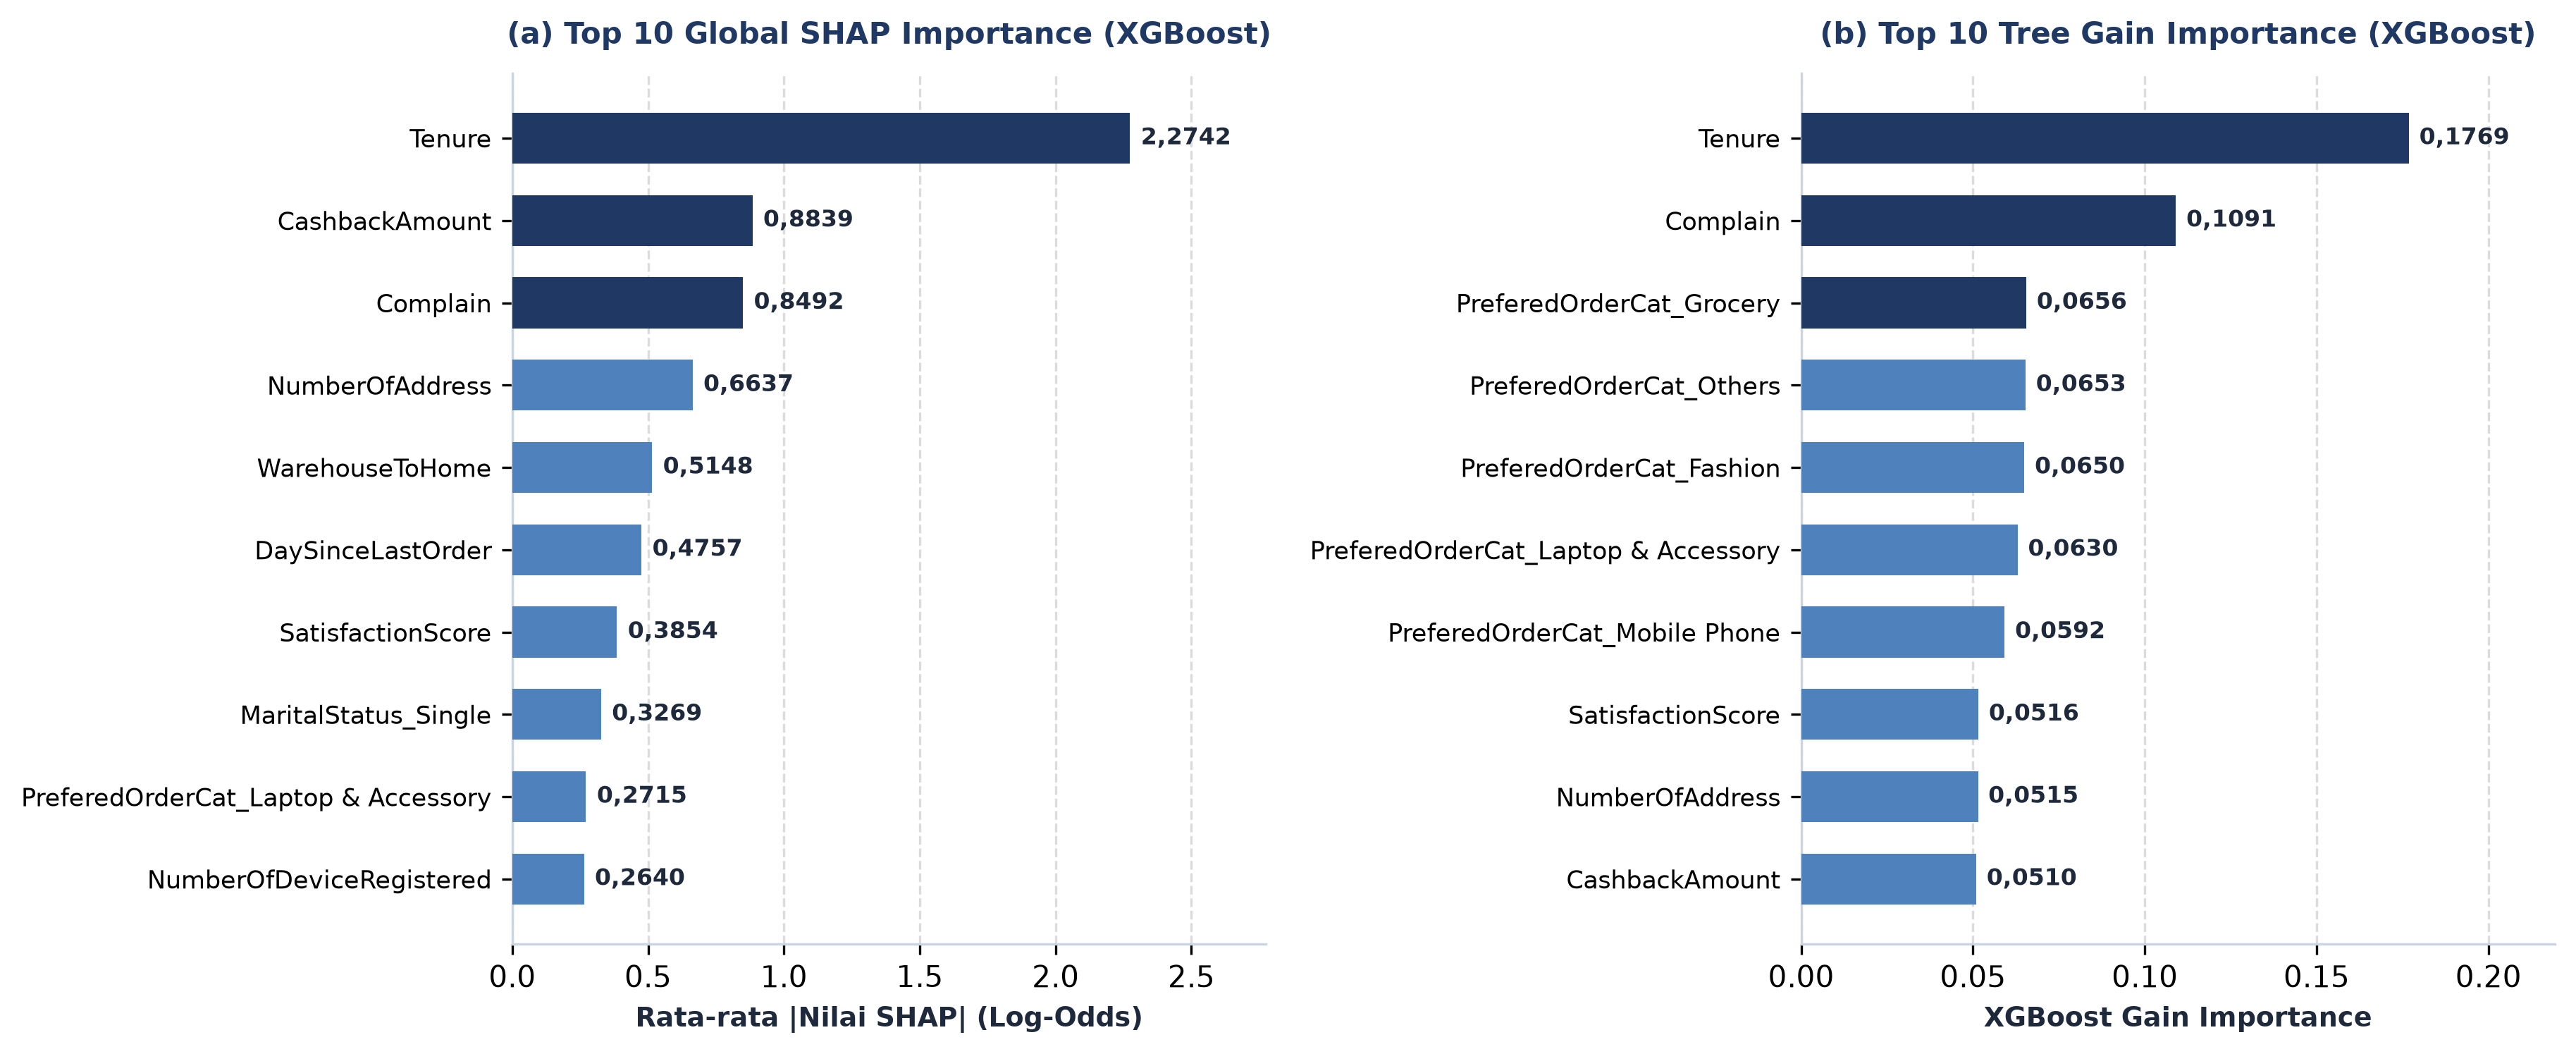
\includegraphics[width=\textwidth]{gambar_4_4_shap_dual_validation.png}
  \caption{Validasi Ganda Top 10 Fitur Dominan: Global SHAP vs XGBoost Gain Importance}
  \label{fig:shap_dual}
\end{figure}

Hasil \textbf{Validasi Ganda} pada Tabel~\ref{tab:dual_val} dan Gambar~\ref{fig:shap_dual} memverifikasi konsistensi sekaligus memperlihatkan keunggulan analitis SHAP dibandingkan \textit{Gain Importance} konvensional:
\begin{enumerate}[leftmargin=0.8cm, itemsep=2pt]
  \item \textbf{Konsistensi Penggerak Utama (\code{Tenure} \& \code{Complain}):} Atribut \code{Tenure} menempati \textbf{peringkat \#1 secara mutlak} pada kedua metode (Mean $|\mathrm{SHAP}| = \mathbf{2{,}2742}$; Gain $= \mathbf{0{,}1769}$), sedangkan \code{Complain} konsisten berada di jajaran tiga besar (\#3 pada SHAP $= \mathbf{0{,}8492}$; \#2 pada Gain $= \mathbf{0{,}1091}$). Hal ini menegaskan bahwa masa langganan awal yang masih pendek serta pengalaman komplain baru-baru ini merupakan sinyal bahaya paling kuat bagi retensi pelanggan, sejalan dengan temuan empiris Khan et al. (2026) dan Inkesar (2026).
  \item \textbf{Perbedaan Karakteristik Pengukuran (SHAP vs Gain):} Pada grafik SHAP, fitur numerik kontinu seperti \code{CashbackAmount} (0,8839 --- peringkat \#2), \code{NumberOfAddress} (0,6637 --- peringkat \#4), \code{WarehouseToHome} (0,5148 --- peringkat \#5), dan \code{DaySinceLastOrder} (0,4757 --- peringkat \#6) memiliki kontribusi besar terhadap probabilitas prediksi tiap pelanggan, sedangkan kategori \textit{one-hot} seperti \code{PreferedOrderCat\_Grocery} justru menempati peringkat tinggi pada \textit{Gain} (\#3) namun peringkat paling bawah pada SHAP (\#16, hanya 0,0071). Perbedaan ini terjadi karena \textit{Gain Importance} mengukur rata-rata penurunan galat per percabangan pohon (yang cenderung membesar pada fitur biner yang jarang muncul tetapi sangat murni ketika terpilih sebagai pemisah), sementara \textbf{SHAP} mengukur kontribusi marjinal nyata rata-rata di seluruh 654 pelanggan uji sehingga lebih akurat mencerminkan dampak perilaku mayoritas basis pelanggan.
  \item \textbf{Mekanisme Penjelasan Lokal Per Pelanggan:} Pada tingkat individual, metode \code{ChurnExplainer.explain\_local()} di dalam \code{src/explainability.py} mengekstrak \textit{base value} $\phi_0$ beserta kontribusi setiap fitur guna ditampilkan sebagai \textit{SHAP Waterfall Plot}, lalu mengelompokkannya menjadi maksimal tiga \textbf{faktor pendorong risiko (\textit{drivers}, $\phi_j > 0$)} dan tiga \textbf{faktor penahan risiko (\textit{protectors}, $\phi_j < 0$)} agar tim CS/CRM segera memahami pemicu spesifik pada setiap profil pelanggan.
\end{enumerate}

\section{Implementasi Sistem \textit{3-Tier Risk Stratification} dan Rancangan Operasional Dashboard}

Untuk menjembatani hasil pemodelan menuju keputusan operasional bisnis, modul \code{src/risk\_engine.py} mengimplementasikan pemisahan fungsi antara ambang klasifikasi biner (\code{CHURN\_CLASS\_THRESHOLD = 0,50} untuk label biner \code{Predicted\_Churn}) dan ambang stratifikasi risiko bisnis berbasis \code{predict\_proba()} yang dikonfigurasi pada \code{src/config.py}. Fungsi \code{classify\_risk(probability)} melayani prediksi pelanggan tunggal pada Modul 1, sedangkan \code{apply\_risk\_to\_batch(customers, probabilities)} memproses prediksi massal pada Modul 2 dengan menambahkan kolom \code{Churn\_Probability}, \code{Predicted\_Churn}, \code{Risk\_Tier}, dan \code{Recommended\_Action} sesuai pemetaan warna dan aksi retensi pada Tabel~\ref{tab:risk_tier}.

Hingga penyusunan laporan tahap ini, seluruh komponen \textit{backend pipeline} (Task 1 s.d. Task 6: konfigurasi, \textit{data loader}, EDA, \textit{preprocessing}, pelatihan \& evaluasi 3 model, \textit{explainability} SHAP, serta \textit{risk engine}) telah selesai diimplementasikan dan terintegrasi pada cabang utama (\code{main}) repositori GitHub. Adapun implementasi antarmuka web interaktif \code{app/streamlit\_app.py} (Task 7 s.d. Task 9) serta notebook dokumentasi akhir (Task 10) berada pada tahap pengembangan lanjutan. Apabila antarmuka Streamlit telah selesai dijalankan, bukti tangkapan layar keempat modul dashboard dapat disisipkan pada Gambar~\ref{fig:streamlit_12} dan Gambar~\ref{fig:streamlit_34}.

\begin{figure}[H]
  \centering
  % Ganti blok tcolorbox berikut dengan \includegraphics[width=\textwidth]{streamlit_modul_1_2.png} setelah Task 7-8 selesai
  \begin{tcolorbox}[screenshotbox]
    \textit{\textbf{[Sisipkan Screenshot Gambar 4.5 --- Tampilan Modul 1 (Prediksi Individual \& SHAP Waterfall) dan Modul 2 (Batch Prediction)]}}\\
    \small\textit{\textcolor{MutedGray}{Jalankan \texttt{streamlit run app/streamlit\_app.py} setelah Task 7--8 selesai lalu sisipkan tangkapan layar di sini.}}
  \end{tcolorbox}
  \caption{Tampilan Modul 1 (Prediksi Individual \& SHAP Waterfall) dan Modul 2 (\textit{Batch Prediction})}
  \label{fig:streamlit_12}
\end{figure}

\begin{figure}[H]
  \centering
  % Ganti blok tcolorbox berikut dengan \includegraphics[width=\textwidth]{streamlit_modul_3_4.png} setelah Task 9 selesai
  \begin{tcolorbox}[screenshotbox]
    \textit{\textbf{[Sisipkan Screenshot Gambar 4.6 --- Tampilan Modul 3 (Analitik Komparasi 3 Model) dan Modul 4 (Ringkasan EDA)]}}\\
    \small\textit{\textcolor{MutedGray}{Sisipkan tangkapan layar Modul 3 \& Modul 4 setelah Task 9 selesai.}}
  \end{tcolorbox}
  \caption{Tampilan Modul 3 (Analitik Komparasi 3 Model) dan Modul 4 (Ringkasan EDA)}
  \label{fig:streamlit_34}
\end{figure}

\section{Pembahasan Implikasi Bisnis, Strategi Retensi CRM, dan Keterbatasan Penelitian}

Dengan menggabungkan temuan EDA (Tabel~\ref{tab:churn_cat}), evaluasi model XGBoost (Tabel~\ref{tab:evaluasi}), dan interpretasi SHAP (Tabel~\ref{tab:dual_val}), tim manajemen dan CRM memperoleh empat rekomendasi strategis berbasis data:
\begin{enumerate}[leftmargin=0.8cm, itemsep=2pt]
  \item \textbf{Program Retensi Intensif Pelanggan Baru (\textit{Onboarding Guard}):} Karena \code{Tenure} merupakan faktor penentu \#1 (Mean $|\mathrm{SHAP}| = 2{,}2742$), risiko perpindahan pelanggan paling tinggi terjadi pada bulan-bulan awal setelah registrasi. Tim pemasaran perlu memfokuskan kampanye \textit{onboarding}, panduan penggunaan, dan penawaran pembelian kedua/ketiga secara agresif pada pelanggan dengan \code{Tenure} $\le 3$ bulan.
  \item \textbf{Percepatan SLA Penanganan Komplain ($< 24$ Jam):} \code{Complain} terbukti menjadi sinyal kritis di posisi \#3 SHAP dan \#2 Gain. Setiap pelanggan yang mengajukan keluhan harus otomatis dipantau; apabila skor probabilitas risikonya melewati ambang \textbf{High Risk} ($p \ge 0{,}65$), tim layanan pelanggan wajib melakukan \textit{service recovery} proaktif beserta kompensasi voucher retensi.
  \item \textbf{Segmentasi Kampanye Kategori \code{Mobile Phone} \& Status \code{Single}:} Segmen \code{Mobile Phone} (\textit{churn rate} 26,90\%) dan pelanggan \code{Single} (25,82\%) memperlihatkan sensitivitas harga serta kecenderungan berpindah platform yang tinggi. Pengiriman notifikasi personalisasi dan promo \textit{cashback} terarah (\textbf{Medium Risk}) lebih efektif dialokasikan pada segmen ini dibandingkan diskon massal kepada segmen \code{Grocery} yang sudah loyal (4,15\%).
  \item \textbf{Optimalisasi Anggaran Insentif \textit{Cashback}:} Nilai \code{CashbackAmount} menempati peringkat \#2 pada SHAP (0,8839), sehingga perubahan besaran insentif \textit{cashback} memiliki daya dorong besar terhadap probabilitas bertahan. Dengan akurasi \textit{Precision} XGBoost sebesar 75,41\% (FPR hanya 5,48\%), anggaran promosi dapat dihemat secara signifikan.
\end{enumerate}

Dari sudut pandang metodologis, terdapat dua \textbf{keterbatasan penelitian} yang perlu dicatat untuk pengembangan berikutnya. \textbf{Pertama}, penerapan bobot kelas \code{scale\_pos\_weight} sebesar 5,1385 efektif mendongkrak \textit{Recall} menjadi 85,98\%, namun secara matematis menggeser keluaran probabilitas mentah (\code{predict\_proba}) ke arah nilai yang lebih tinggi dibandingkan prevalensi \textit{churn} aktual (16,30\%). Akibatnya, jumlah pelanggan yang masuk kategori \textit{High Risk} ($p \ge 0{,}65$) berpotensi relatif besar bila ambang batas tidak disesuaikan atau dikalibrasi ulang. \textbf{Kedua}, dataset aktual belum mencakup variabel nilai moneter total transaksi (\textit{gross merchandise value}) maupun riwayat interaksi sesi web (\textit{clickstream}), sehingga estimasi kerugian finansial per pelanggan (\textit{customer lifetime value}) belum dapat dihitung secara langsung di dalam \textit{risk engine}.

% ============================================================
% BAB 5: KESIMPULAN DAN SARAN
% ============================================================
\chapter{Kesimpulan dan Saran}

\section{Kesimpulan}

Berdasarkan perancangan, implementasi, serta evaluasi eksperimen yang telah dilaksanakan, diperoleh empat kesimpulan utama yang menjawab seluruh rumusan masalah proyek:
\begin{enumerate}[leftmargin=0.8cm, itemsep=2pt]
  \item \textbf{Protokol Anti-\textit{Data Leakage} dan Penanganan Imbalance Alami:} Alur \textit{preprocessing} yang menerapkan standarisasi kategori deterministik, eliminasi \textbf{672 baris duplikat} sebelum pemisahan data (dari 3.941 menjadi 3.269 baris unik), \textit{Stratified Train-Test Split} 80:20 (2.615 latih : 654 uji), serta pembungkusan \code{SimpleImputer}, \code{OneHotEncoder}, dan \code{StandardScaler} di dalam \code{ColumnTransformer} berhasil menjamin tidak adanya kebocoran data. Penanganan ketidakseimbangan kelas (rasio 5,13 : 1) melalui \textit{cost-sensitive learning} (\code{class\_weight='balanced'} dan \code{scale\_pos\_weight = 5,1385}) tanpa SMOTE terbukti mampu mencapai \textit{Recall} di atas 85\% pada seluruh model dengan tetap mempertahankan distribusi perilaku pelanggan yang alami.
  \item \textbf{Performa Komparatif Tiga Model Klasifikasi:} Hasil pengujian pada \textit{held-out test set} (654 baris) membuktikan bahwa model \textit{tree-ensemble} jauh lebih unggul dibandingkan \textit{baseline} linear dalam menangkap pola non-linear perilaku pelanggan. \textbf{XGBoost} meraih performa terbaik dengan \textbf{F1-Score 80,35\%}, \textbf{ROC-AUC 0,9665}, \textbf{Accuracy 93,12\%}, \textbf{Precision 75,41\%}, \textbf{Recall 85,98\%}, dan \textbf{Specificity 94,52\%} (FPR 5,48\%), mengungguli \textbf{Random Forest} (F1-Score 78,11\%; ROC-AUC 0,9636) dan \textbf{Logistic Regression} (F1-Score 58,43\%; ROC-AUC 0,9194; Recall 90,65\% namun menghasilkan 128 \textit{False Positive}).
  \item \textbf{Faktor Dominan Berbasis SHAP dan Validasi Ganda:} Analisis \textit{Global SHAP Importance} pada model XGBoost mengidentifikasi lima faktor pendorong utama \textit{churn}, yaitu \code{Tenure} (Mean $|\mathrm{SHAP}| = 2{,}2742$), \code{CashbackAmount} (0,8839), \code{Complain} (0,8492), \code{NumberOfAddress} (0,6637), dan \code{WarehouseToHome} (0,5148). Melalui \textbf{Validasi Ganda}, \code{Tenure} dan \code{Complain} terbukti konsisten menempati posisi puncak baik pada SHAP maupun \textit{XGBoost Gain Importance}, sementara temuan EDA menegaskan kerentanan tertinggi pada kategori \textbf{Mobile Phone} (26,90\%) dan pelanggan \textbf{Single} (25,82\%).
  \item \textbf{Operasionalisasi ke Dalam Mesin Stratifikasi Risiko:} Model terbaik (\code{best\_model\_pipeline.joblib}), modul penjelasan lokal \& global (\code{src/explainability.py}), serta aturan pemetaan probabilitas menjadi tiga kategori risiko (\textbf{High Risk} $\ge 0{,}65$; \textbf{Medium Risk} $0{,}35\text{--}0{,}64$; \textbf{Low Risk} $< 0{,}35$ pada \code{src/risk\_engine.py}) telah siap dioperasionalisasikan untuk mendukung pengambilan keputusan retensi tim CRM pada antarmuka \textit{web dashboard} Streamlit.
\end{enumerate}

\section{Saran}

Untuk penyempurnaan implementasi sistem maupun penelitian lanjutan di masa mendatang, tim mengajukan tiga saran strategis:
\begin{enumerate}[leftmargin=0.8cm, itemsep=2pt]
  \item \textbf{Kalibrasi Probabilitas Pascapembobotan Kelas:} Mengingat penggunaan \code{scale\_pos\_weight} menggeser distribusi skor probabilitas ke atas, pada implementasi produksi disarankan menerapkan kalibrasi probabilitas (seperti \textit{Platt Scaling} atau \textit{Isotonic Regression}) menggunakan \code{CalibratedClassifierCV} agar nilai probabilitas pada ambang batas \textit{3-Tier Risk Stratification} (0,35 dan 0,65) selaras secara statistik dengan rasio \textit{churn} riil perusahaan.
  \item \textbf{Pengayaan Atribut Transaksional dan Telemetri Sesi Web:} Merujuk pada kerangka kerja Khan et al. (2026), integrasi fitur tambahan seperti rata-rata nilai transaksi (\textit{monetary value}), tingkat pengabaian keranjang belanja (\textit{cart abandonment rate}), serta kualitas pengalaman pengguna situs akan meningkatkan ketajaman prediksi sekaligus memungkinkan perhitungan dampak finansial langsung (\textit{expected value of retention}).
  \item \textbf{Penyelesaian Antarmuka Streamlit dan Pemantauan \textit{Data Drift}:} Menyelesaikan integrasi visual antarmuka 4 modul pada \code{app/streamlit\_app.py} (Task 7--9) serta menyertakan mekanisme pemantauan \textit{data drift} dan \textit{concept drift} secara berkala agar model tetap akurat menghadapi perubahan perilaku konsumen \textit{e-commerce} di masa depan.
\end{enumerate}

% ============================================================
% DAFTAR PUSTAKA (APA 7TH EDITION)
% ============================================================
\clearpage
\phantomsection
\addcontentsline{toc}{chapter}{DAFTAR PUSTAKA}
\begin{center}
  {\fontsize{14}{17}\selectfont\bfseries DAFTAR PUSTAKA\par}
\end{center}
\vspace{8pt}

\begingroup
\fontsize{11.5}{16.5}\selectfont
\setlength{\parindent}{0pt}
\setlength{\parskip}{6pt}
\newcommand{\bibentry}[1]{\par\hangindent=1.27cm\hangafter=1 #1\par}

\bibentry{Ahmad, N., Awan, M. J., Nobanee, H., Zain, A. M., Naseem, A., \& Mahmoud, A. (2024). Customer personality analysis for churn prediction using hybrid ensemble models and class balancing techniques. \textit{IEEE Access}, 12, 1865--1879. \url{https://doi.org/10.1109/ACCESS.2023.3334641}}

\bibentry{Breiman, L. (2001). Random forests. \textit{Machine Learning}, 45(1), 5--32. \url{https://doi.org/10.1023/A:1010933404324}}

\bibentry{Chen, T., \& Guestrin, C. (2016). XGBoost: A scalable tree boosting system. In \textit{Proceedings of the 22nd ACM SIGKDD International Conference on Knowledge Discovery and Data Mining} (pp. 785--794). \url{https://doi.org/10.1145/2939672.2939785}}

\bibentry{Hantash, L. A., Whitmore, O., Muzaffar, M., Izquierdo Mayorga, L. J., Sucandrawati, N. L. K. A. S., \& Van, S. H. (2026). AI-driven customer churn prediction and retention intelligence from behavioral signals. \textit{Journal of Intelligent Decision Making and Information Science}, 3(7s), 1023--1041. \url{https://doi.org/10.59543/jidmis.v3.1785}}

\bibentry{Inkesar, A. (2026). An explainable machine learning approach with density-regularized oversampling for industrial customer churn prediction. \textit{IEEE Access}, 14, 119355--119383. \url{https://doi.org/10.1109/ACCESS.2026.3718205}}

\bibentry{Khan, M. I., Dewan, M. A., Ahmed, K. R., Jamee, S. S., Reon, M. A. H., Bhuiyan, M. S., \& Rahman, M. N. (2026). WPIS: Machine learning-driven e-commerce churn prediction integrating technical metrics and information quality for strategic MIS decision support. \textit{Information}, 17(9), 886. \url{https://doi.org/10.3390/info17090886}}

\bibentry{Lundberg, S. M., \& Lee, S.-I. (2017). A unified approach to interpreting model predictions. \textit{Advances in Neural Information Processing Systems}, 30, 4765--4774.}
\endgroup

\end{document}
